%\documentclass[11pt,leqno]{book}
%\usepackage[spanish,activeacute]{babel}
%\usepackage[utf8]{inputenc}
%\usepackage{enumerate}
%
%\begin{document}

\chapter{Desarrollo informático}
\label{ch:informatica}

Para la realización de todos los experimentos en este capítulo (con excepción de los test estadísticos ANOVA y rangos múltiples, hechos en una versión de prueba de Statgraphics) se ha utilizado el software \texttt{R} junto con los paquetes \texttt{bmp} para leer imágenes en formato \textit{.bmp} y \texttt{gdpc} cuya versión en desarrollo puede encontrarse en el enlace en \cite{ezeq}. El resto de funciones utilizadas están en paquetes que se instalan en una instalación por defecto en \texttt{R}.

\section{Breve descripción del paquete utilizado}
y de las funciones que has hecho tú.

\section{Estudio de tiempos en función de los parámetros}


\section{Aplicación: Compresión de imágenes}

Vamos a ver como primera aplicación la compresión de imágenes tanto en escala de grises como a color. Se ha elegido esta aplicación porque las imágenes tienen la propiedad de que cada pixel se parece a los píxeles que tiene alrededor, de forma que si tomamos como cada serie temporal cada fila o columna de una imagen tenemos que las series se van a ir pareciendo entre sí, permitiendo obtener, en principio, pocas componentes principales con respecto al tamaño de la imagen y así tener un alto factor de compresión (que no es más que la reducción de dimensión de las series originales: las filas o columnas de la imagen).\\

Para aplicar el algoritmo GDPC (Generalized Dynamic Principal Components) a imágenes, se toman por tanto las columnas (o las filas) de una imagen como series temporales. El paquete \texttt{gdpc}, dada una matriz, toma como series temporales las columnas, por lo que a no ser que se especifique lo contrario, vamos a coger las columnas de la imagen como series temporales. De esta forma si la matriz tiene 500 filas por 300 columnas, tendríamos 300 series de 500 valores cada una. Para aplicar esto a imágenes a color, se toma cada capa R, G y B de la imagen a color como una matriz distinta y se sacan las componentes principales de cada matriz. Se han hecho experimentos con las siguientes tres imágenes, todas en formato \textit{.bmp} para que no hubiera una previa compresión de las mismas:
\begin{figure}[H]
 \centering
  \subfloat[Lena]{
   \label{f:lena}
    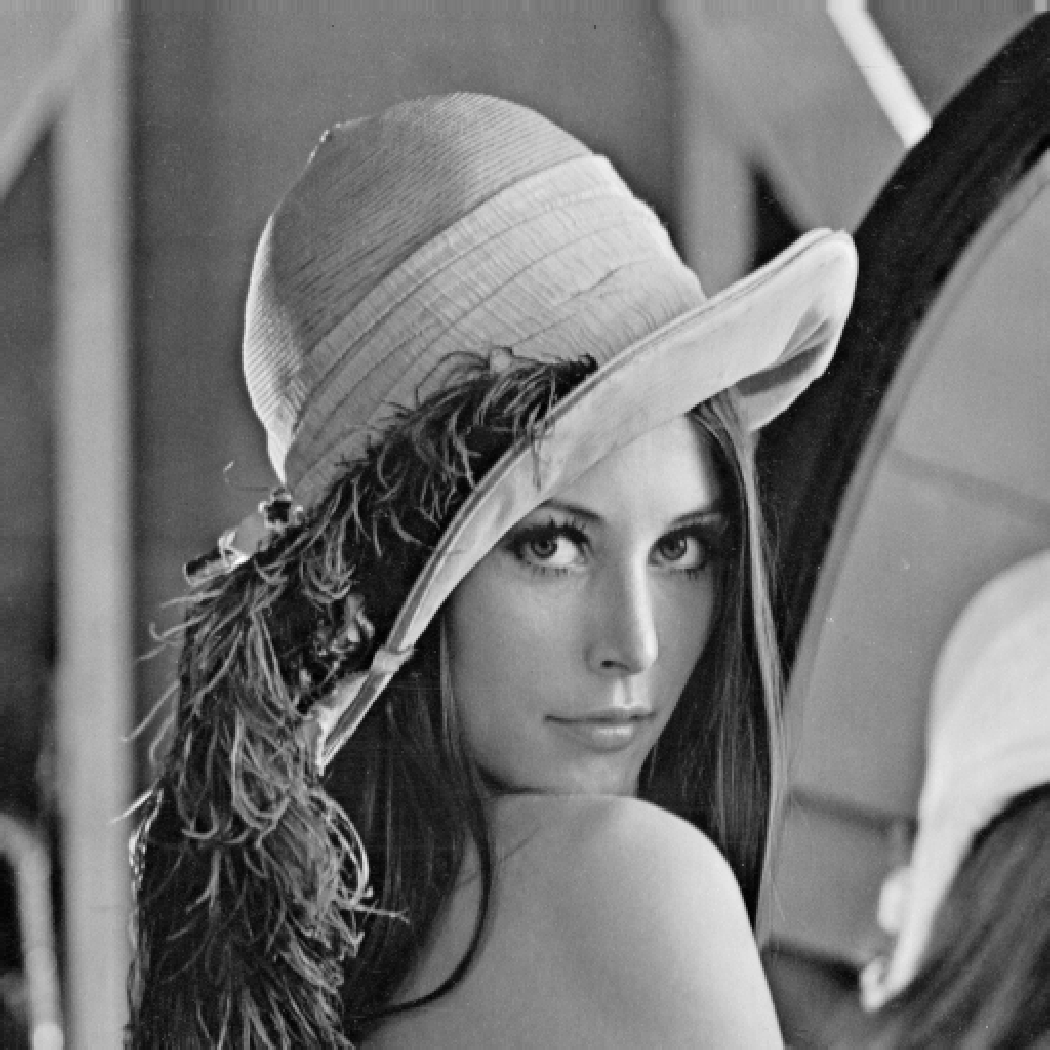
\includegraphics[width=0.32\textwidth]{../imagenes/LenaOriginal.pdf}}
  \subfloat[Pato]{
   \label{f:pato}
    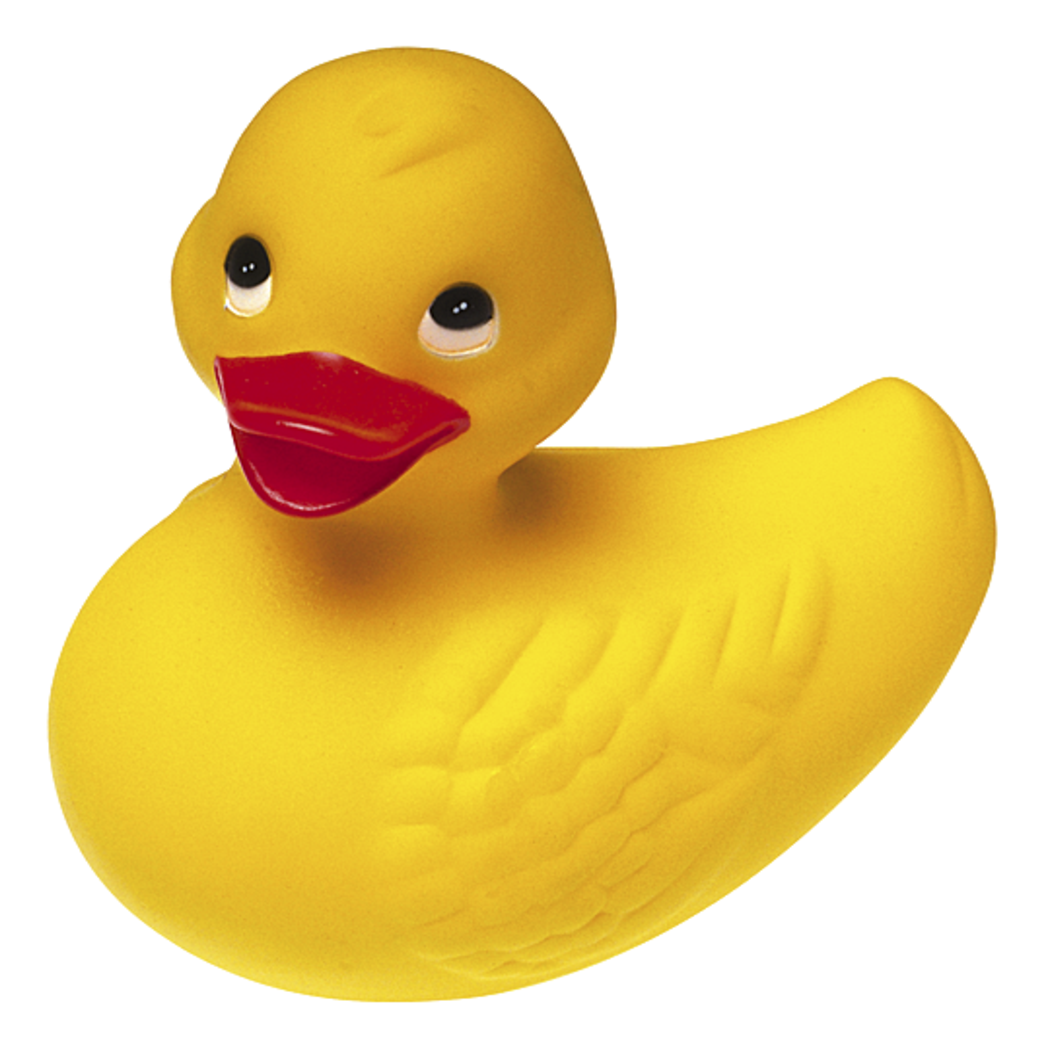
\includegraphics[width=0.32\textwidth]{../imagenes/duckOriginal.pdf}}
  \subfloat[Tigre]{
   \label{f:tigre}
    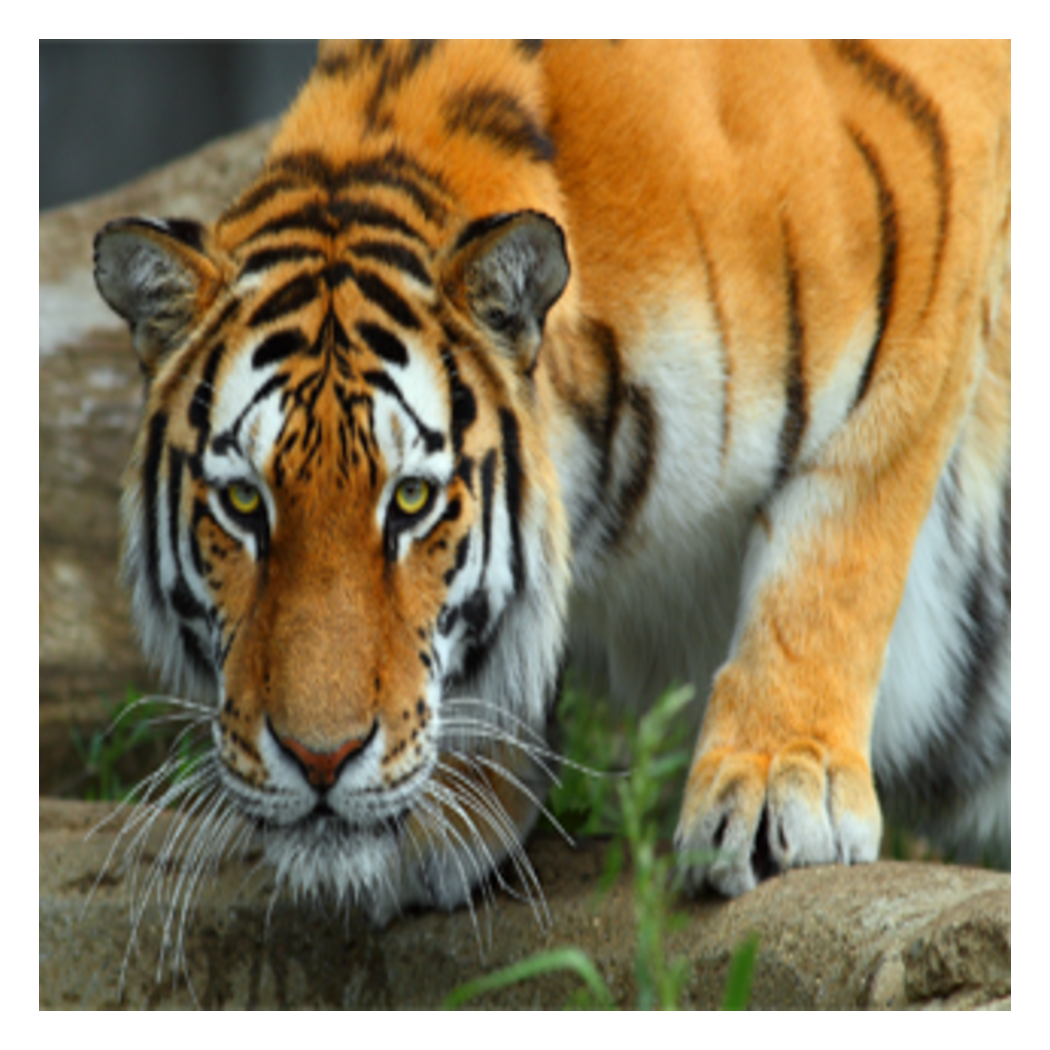
\includegraphics[width=0.34\textwidth]{../imagenes/tigerOriginal.pdf}}
 \caption{Imágenes utilizadas}
 \label{f:imgs}
\end{figure}

Se han elegido las tres imágenes anteriores por las siguientes razones:
\begin{enumerate}
\item Hay una en escala de grises y dos a color, por lo que se ha podido experimentar con imágenes a color, que presentan 3 matrices distintas, una para cada canal de color.
\item Hay una imagen más sencilla, la del pato, y dos con más detalles, para comprobar cómo se comporta el algoritmo en cada caso.
\item Hay dos imágenes más grandes (Lena es de 512x512 y la del pato de 500x546) y una más pequeña, la del tigre, que tiene 320x240.
\end{enumerate}

Intuitivamente, en el primer punto deberíamos obtener que la imagen reconstruida en escala de grises tiene más calidad que las imágenes en color, puesto que al reconstruir tres capas en lugar de una hay más posibilidad de perder información general a la hora de ver la imagen. Del mismo modo, en el segundo punto se debería obtener que la imagen más sencilla tiene más calidad que las otras dos, ya que debe ser más fácil reconstruir una serie prácticamente constante.\\ %En cuanto al tercer punto, parecería lógico pensar que cuanto más pequeña sea la imagen más fácil será de reconstruir, ya que \\

En un primer experimento, se han sacado las componentes principales con \texttt{k\_max = 5} y \texttt{expl\_var = 0.95} en los tres casos y se han reconstruido las imágenes con las componentes y los coeficientes obtenidos. En el caso de las imágenes a color se han separado los canales de color, sacado las componentes principales para cada canal, se ha reconstruido cada canal con sus componentes y se han vuelto a juntar para guardar la imagen. En el caso de la imagen de Lena, se han obtenido 12 componentes principales dinámicas. Para el pato se han obtenido 6, 5 y 6 para las capas R, G y B, respectivamente, y para el tigre 10, 13 y 11. Los resultados obtenidos han sido los mostrados en las figuras \ref{f:imgsLena}, \ref{f:imgsPato} y \ref{f:imgsTigre}.\\

Es conveniente notar que para poder mostrar las imágenes ha habido que reescalar los valores obtenidos por la reconstrucción de las series a los intervalos $[0,255]$ en el caso de imágenes en blanco y negro y a $[0,1]$ en cada capa en el caso de imágenes a color. Esto ha sido así por las dos funciones de \texttt{R} que se han utilizado para dibujar las imágenes, \texttt{image()} para el primer caso y \texttt{rasterImage()} para el segundo. En \texttt{image()} se umbralizan directamente los valores que superan el 255 o que están por debajo del 0, sin embargo \texttt{rasterImage()} no, por lo que se ha procedido a hacerlo manualmente. En este caso no se podía umbralizar porque las capas originales estaban en el intervalo $[0,255]$ por lo que se ha utilizado el homeomorfismo de cambio del intervalo $[\text{min},\text{max}]$ al intervalo $[0,1]$:
\[	x^{'} = \frac{x - \text{min}}{\text{max}-\text{min}} 	\]
con $x \in [\text{min},\text{max}]$.

\begin{figure}[H]
 \centering
  \subfloat[Imagen original]{
   \label{f:lenaO}
    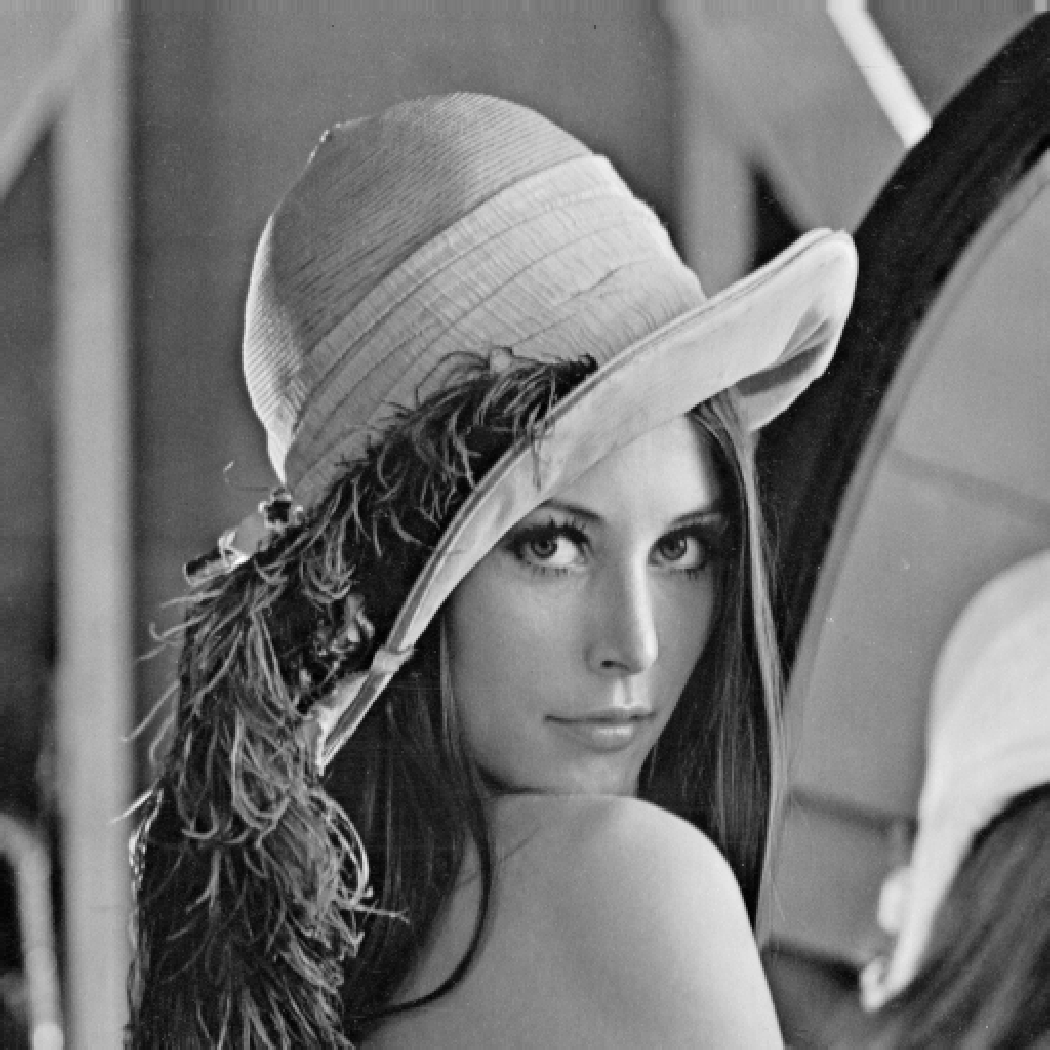
\includegraphics[width=0.5\textwidth]{../imagenes/LenaOriginal.pdf}}
  \subfloat[Imagen reconstruida]{
   \label{f:lenaR}
    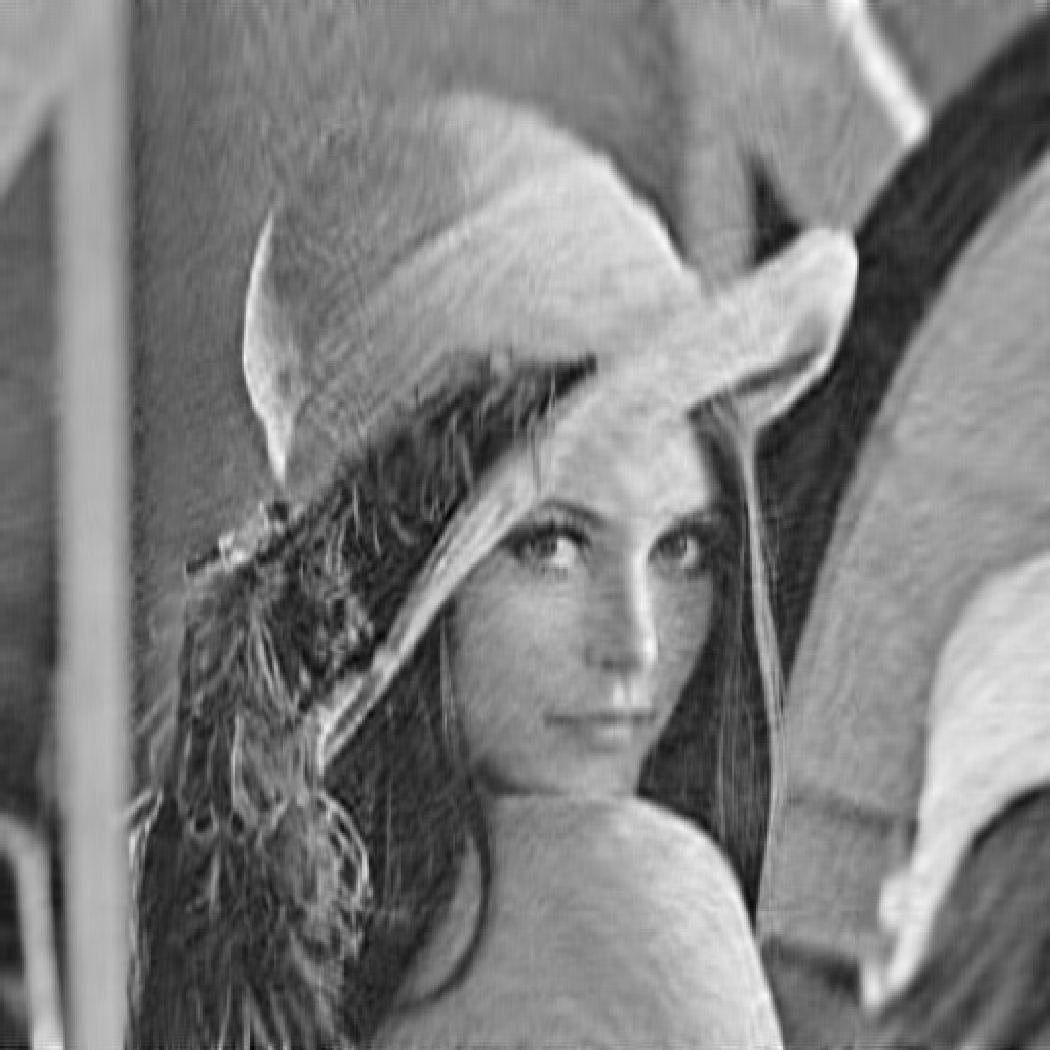
\includegraphics[width=0.5\textwidth]{../imagenes/lena095.pdf}}
 \caption{Lena}
 \label{f:imgsLena}
\end{figure}

\begin{figure}
 \centering
  \subfloat[Imagen original]{
   \label{f:patoO}
    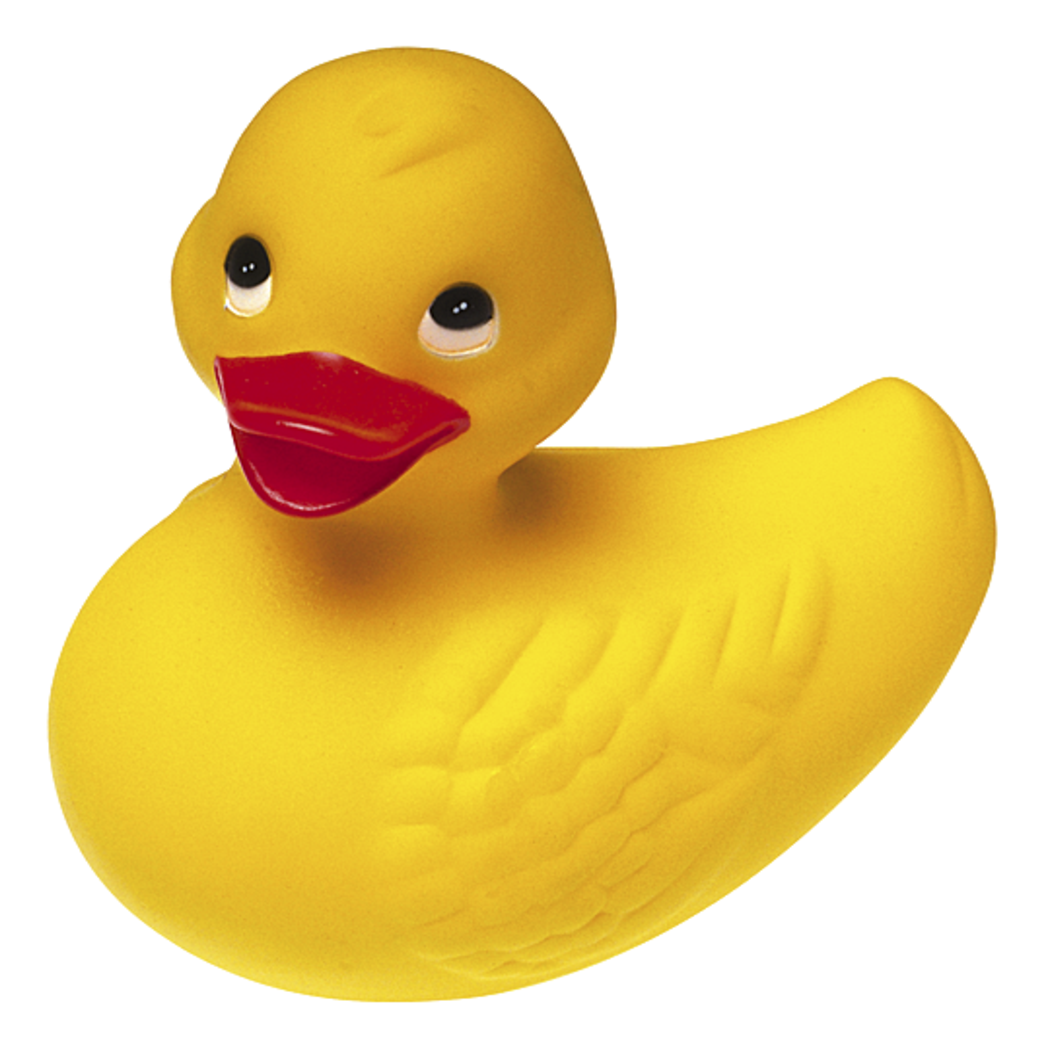
\includegraphics[width=0.5\textwidth]{../imagenes/duckOriginal.pdf}}
  \subfloat[Imagen reconstruida]{
   \label{f:patoR}
    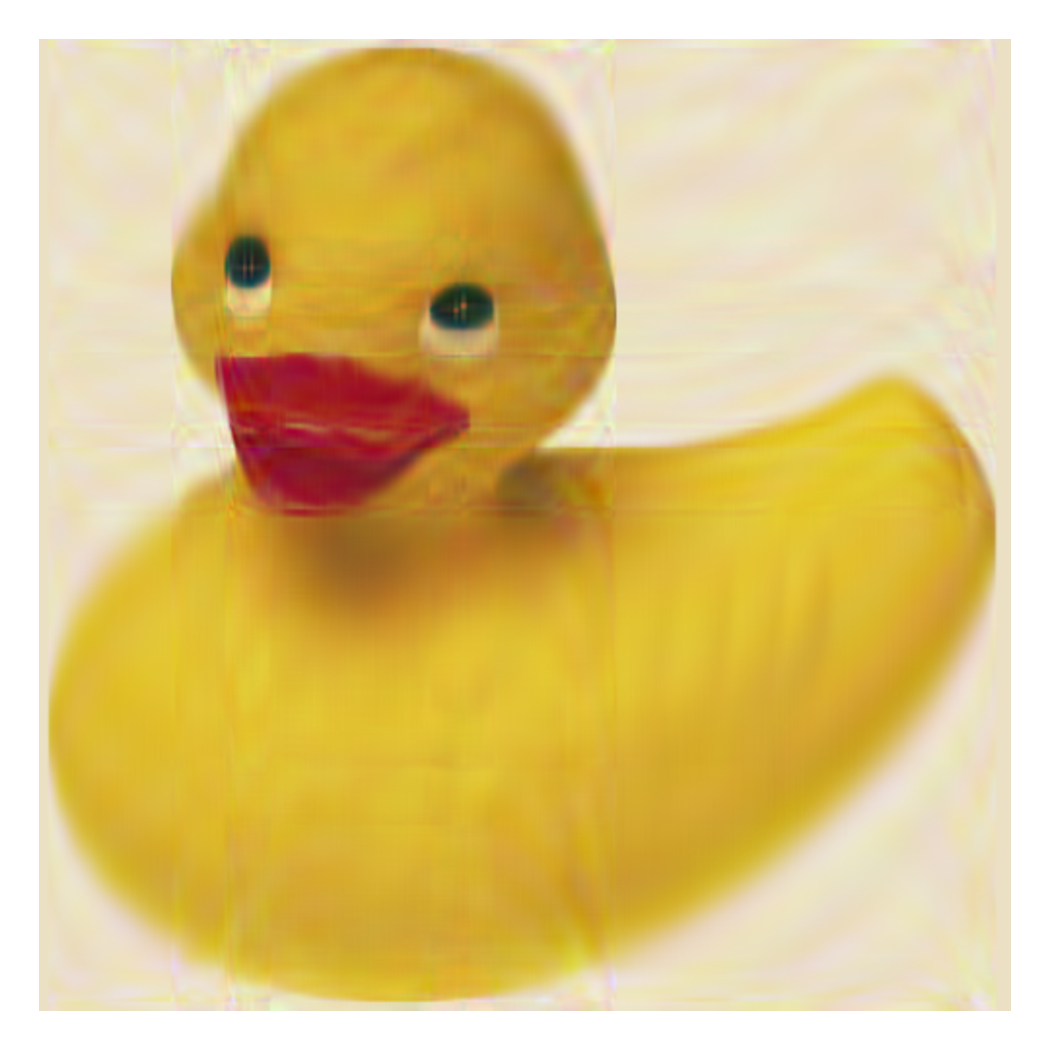
\includegraphics[width=0.5\textwidth]{../imagenes/duck095.pdf}}
 \caption{Pato}
 \label{f:imgsPato}
\end{figure}

\begin{figure}
 \centering
  \subfloat[Imagen original]{
   \label{f:tigreO}
    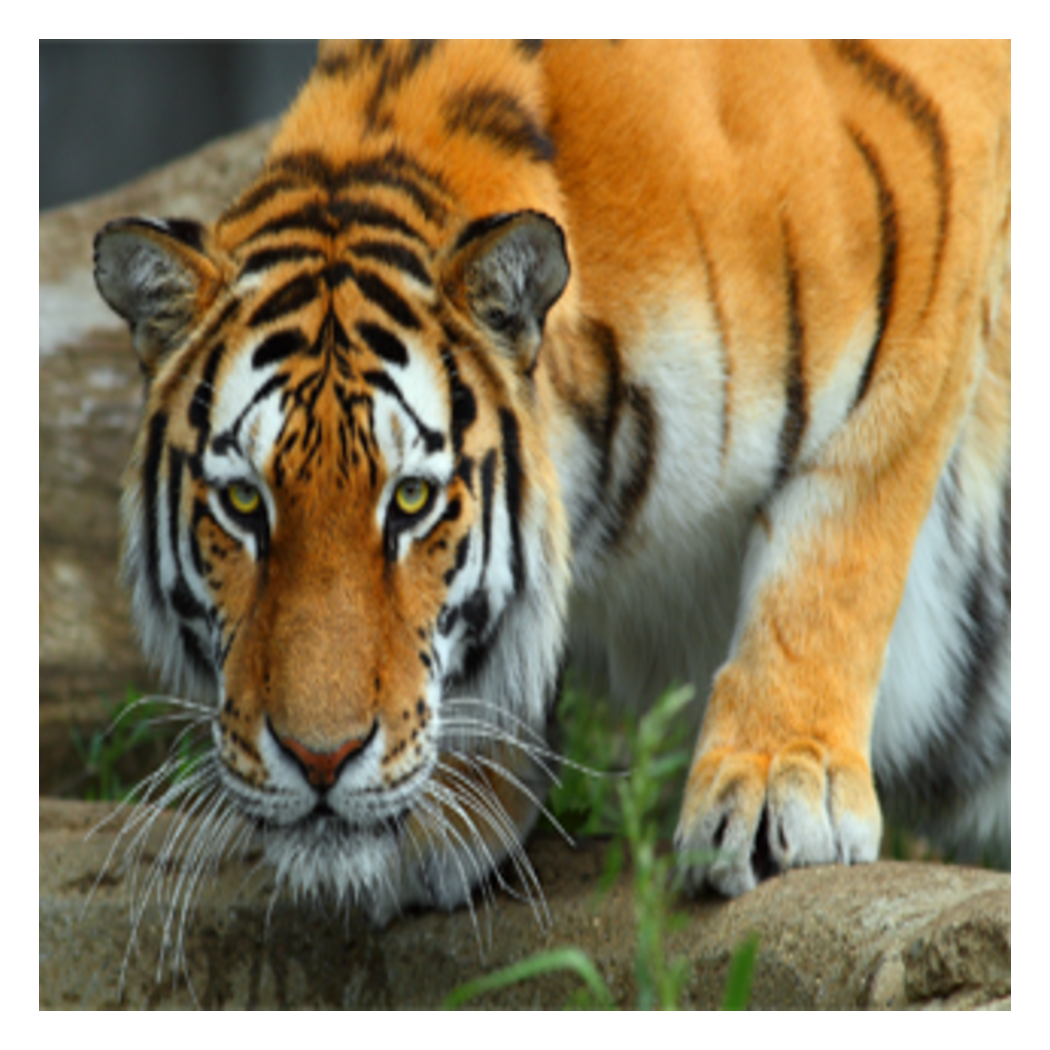
\includegraphics[width=0.5\textwidth]{../imagenes/tigerOriginal.pdf}}
  \subfloat[Imagen reconstruida]{
   \label{f:tigreR}
    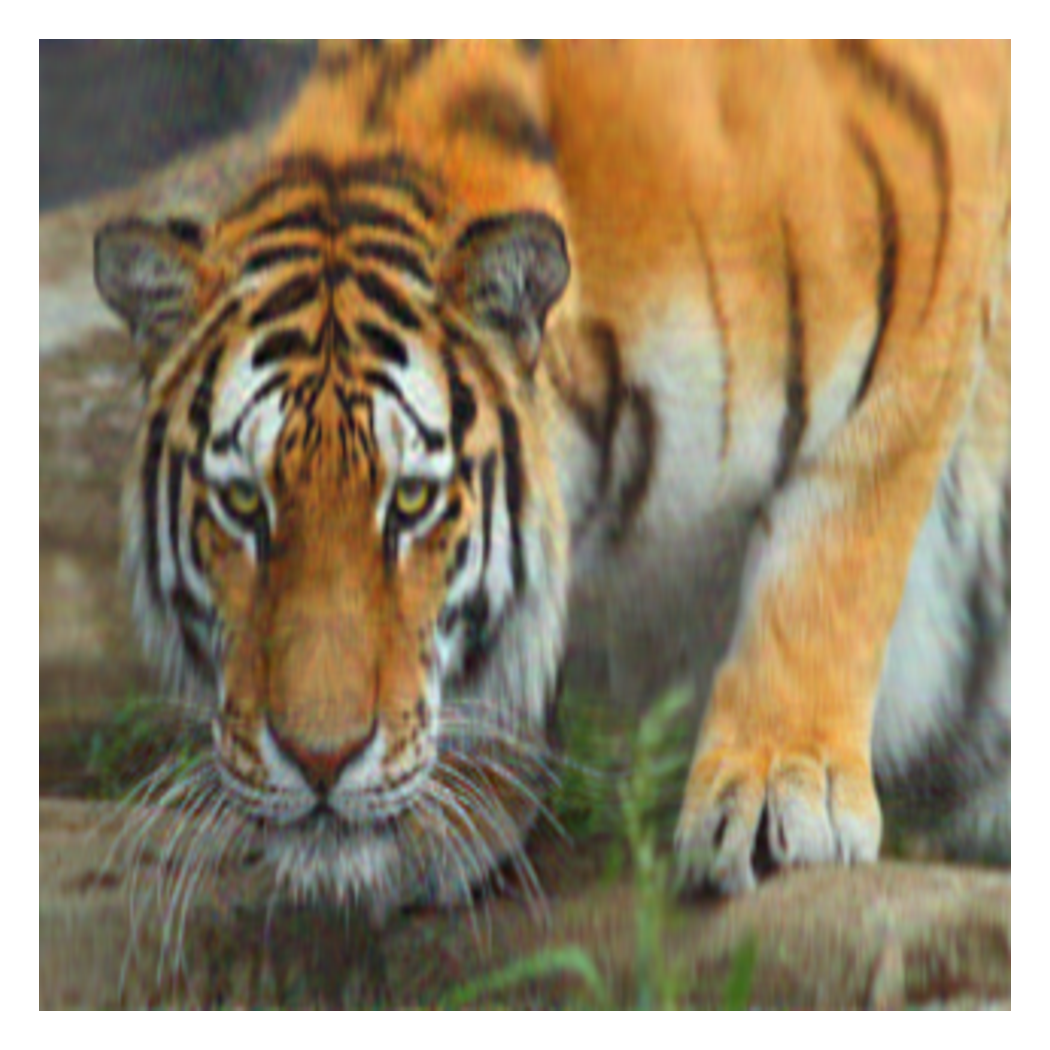
\includegraphics[width=0.5\textwidth]{../imagenes/tiger.pdf}}
 \caption{Tigre}
 \label{f:imgsTigre}
\end{figure}


Con estos experimentos podemos ver que en cuanto al segundo punto, las imágenes más simples no tienen por qué reconstruirse mejor, en contra de lo que se pensaba inicialmente, ya que la imagen más simple, que es la del pato, es la que peor se ve una vez se reconstruye. Esto es debido a que la mayor parte de las series en esa imagen (es decir, las columnas) son muy parecidas. De hecho, las componentes necesarias para explicar el 95\% de la varianza en esta imagen han sido menores que en las otras dos imágenes, concretamente la mitad de las componentes obtenidas con la imagen de Lena, que tiene casi la misma dimensión que la del pato, como se ha comentado antes. Esto implica que si los cambios en la imagen son pequeños (entendiendo como pequeños cambios suaves en el tono o color de la misma) normalmente se van a perder en la reconstrucción. Esto es lo que pasa por ejemplo con la parte del cuerpo del pato, donde está el detalle de las plumas. El cambio es demasiado suave entre todo el fondo amarillo y no es posible recogerlo en tan pocas componentes. Por esto, si los cambios son bruscos y las series difieren unas de otras harán falta más componentes para explicar el mismo porcentaje de varianza y por tanto el algoritmo tardará más pero también será mejor la reconstrucción. De esta forma, se explica que la imagen que peor se ve con respecto a la original sea la del pato, ya que tanto la de Lena como la del tigre tienen cambios más bruscos. De hecho, las partes de la imagen de Lena que son más uniformes en la imagen original se ven un poco peor en la imagen reconstruida.\\

Para ver esto más claro se ha cogido la imagen de Lena y se han hecho cambios en los niveles para pasar de una imagen prácticamente en negro a la imagen original. En este caso se ha hecho explicando el 90\% de varianza para reducir los tiempos de cómputo. Los resultados se pueden ver en las figuras \ref{f:imgsLenaN2}, \ref{f:imgsLenaN3}, \ref{f:imgsLenaN4}, \ref{f:imgsLenaN5} y \ref{f:imgsLenaN6}.\\

\begin{figure}
 \centering
  \subfloat[Imagen original]{
   \label{f:lenaN2O}
    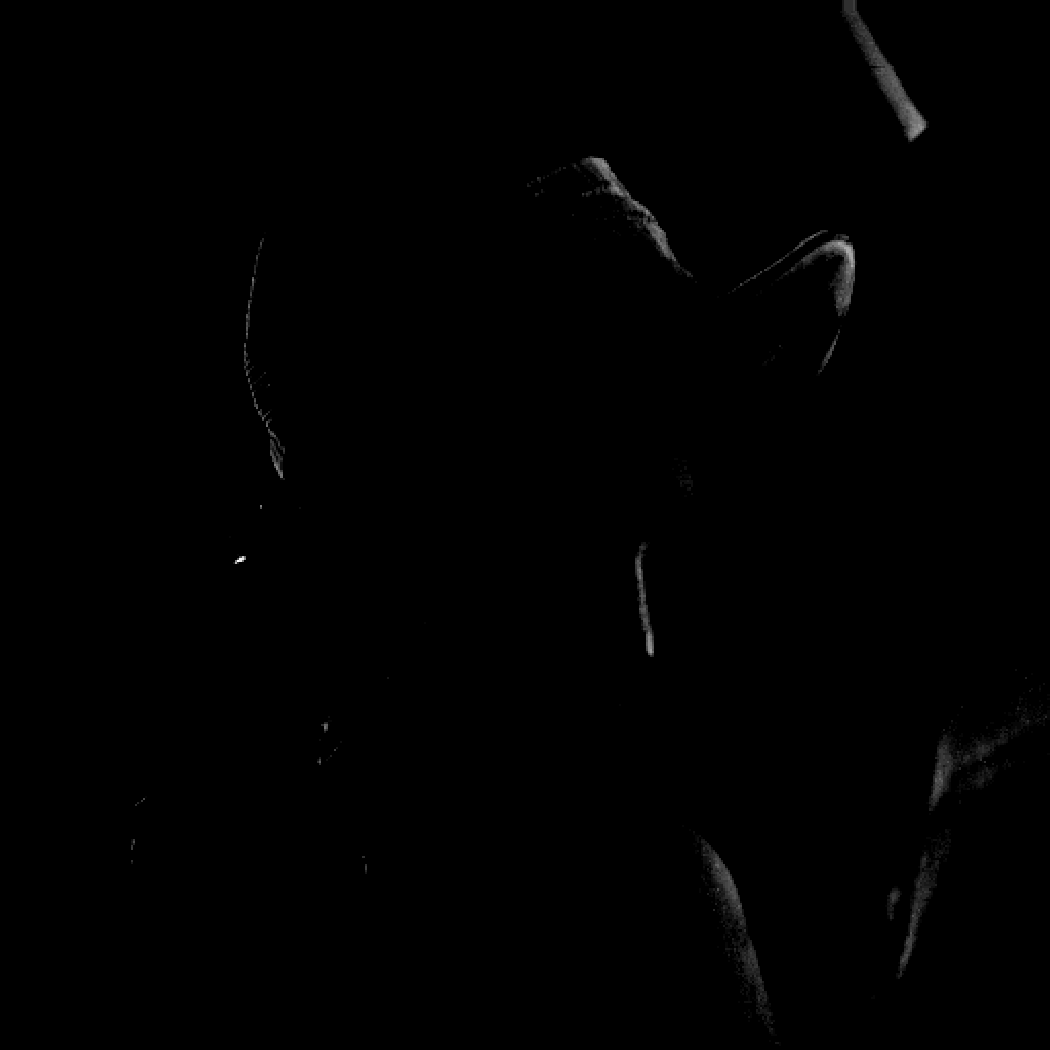
\includegraphics[width=0.5\textwidth]{../imagenes/nivelesLena2.pdf}}
  \subfloat[Imagen reconstruida]{
   \label{f:lenaN2R}
    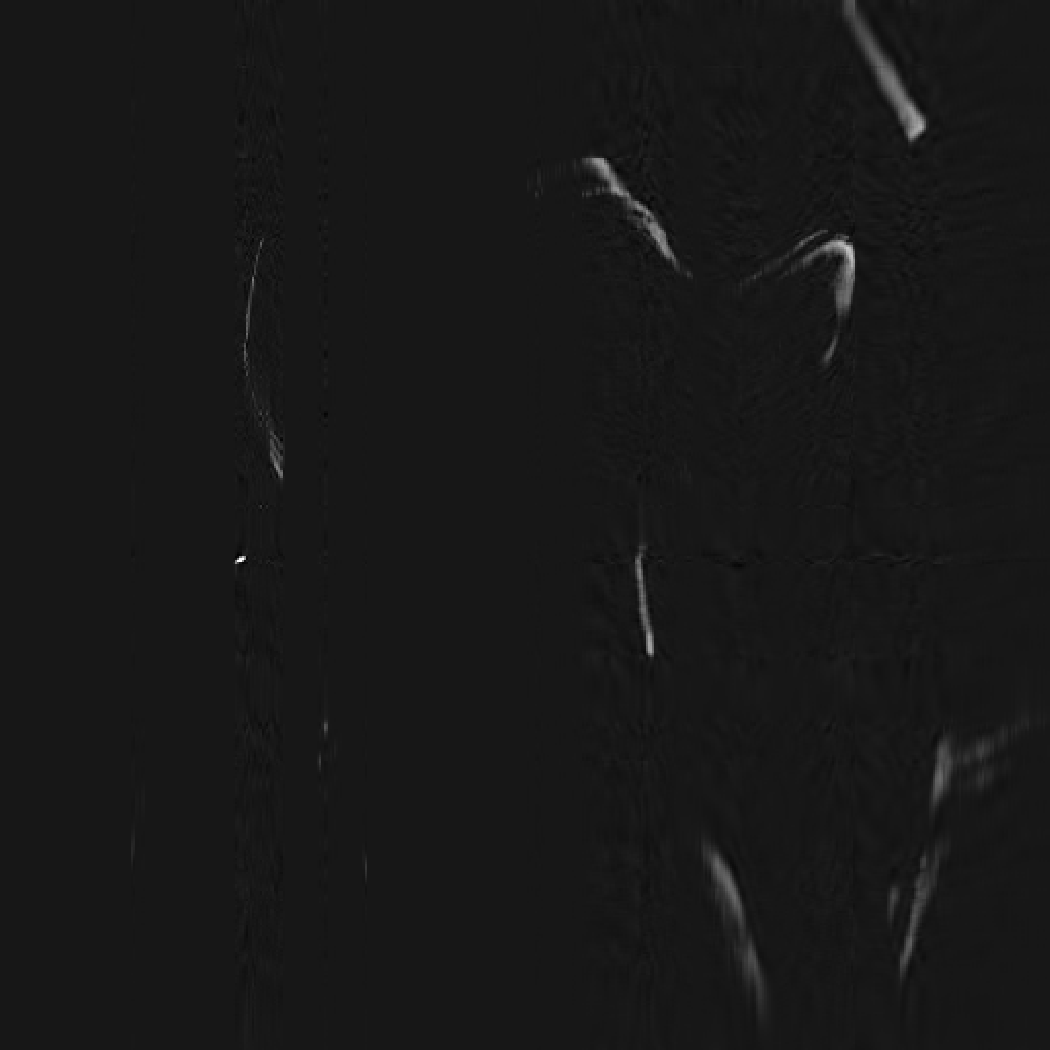
\includegraphics[width=0.5\textwidth]{../imagenes/nivelesLena2r.pdf}}
 \caption{Niveles de Lena}
 \label{f:imgsLenaN2}
\end{figure}

\begin{figure}
 \centering
  \subfloat[Imagen original]{
   \label{f:lenaN3O}
    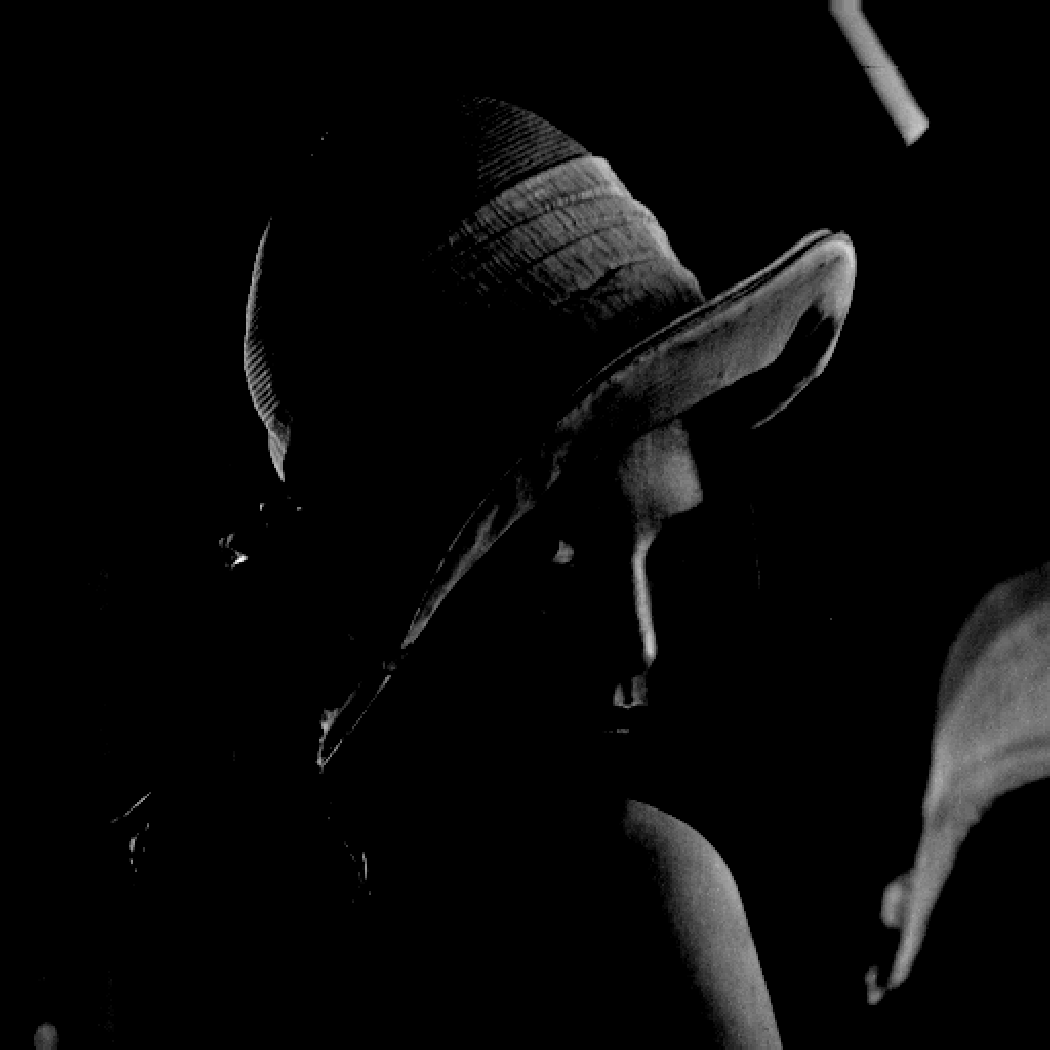
\includegraphics[width=0.5\textwidth]{../imagenes/nivelesLena3.pdf}}
  \subfloat[Imagen reconstruida]{
   \label{f:lenaN3R}
    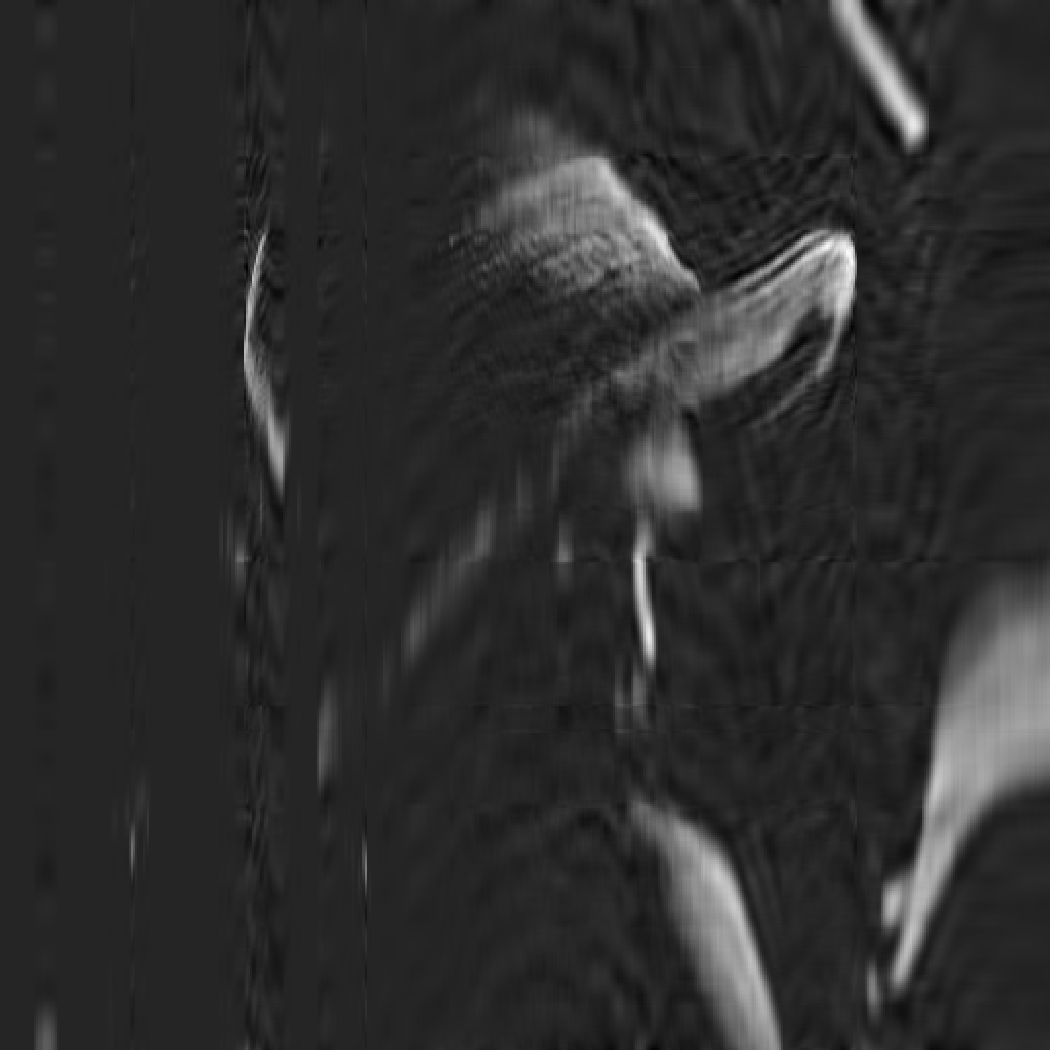
\includegraphics[width=0.5\textwidth]{../imagenes/nivelesLena3r.pdf}}
 \caption{Niveles de Lena}
 \label{f:imgsLenaN3}
\end{figure}

\begin{figure}
 \centering
  \subfloat[Imagen original]{
   \label{f:lenaN4O}
    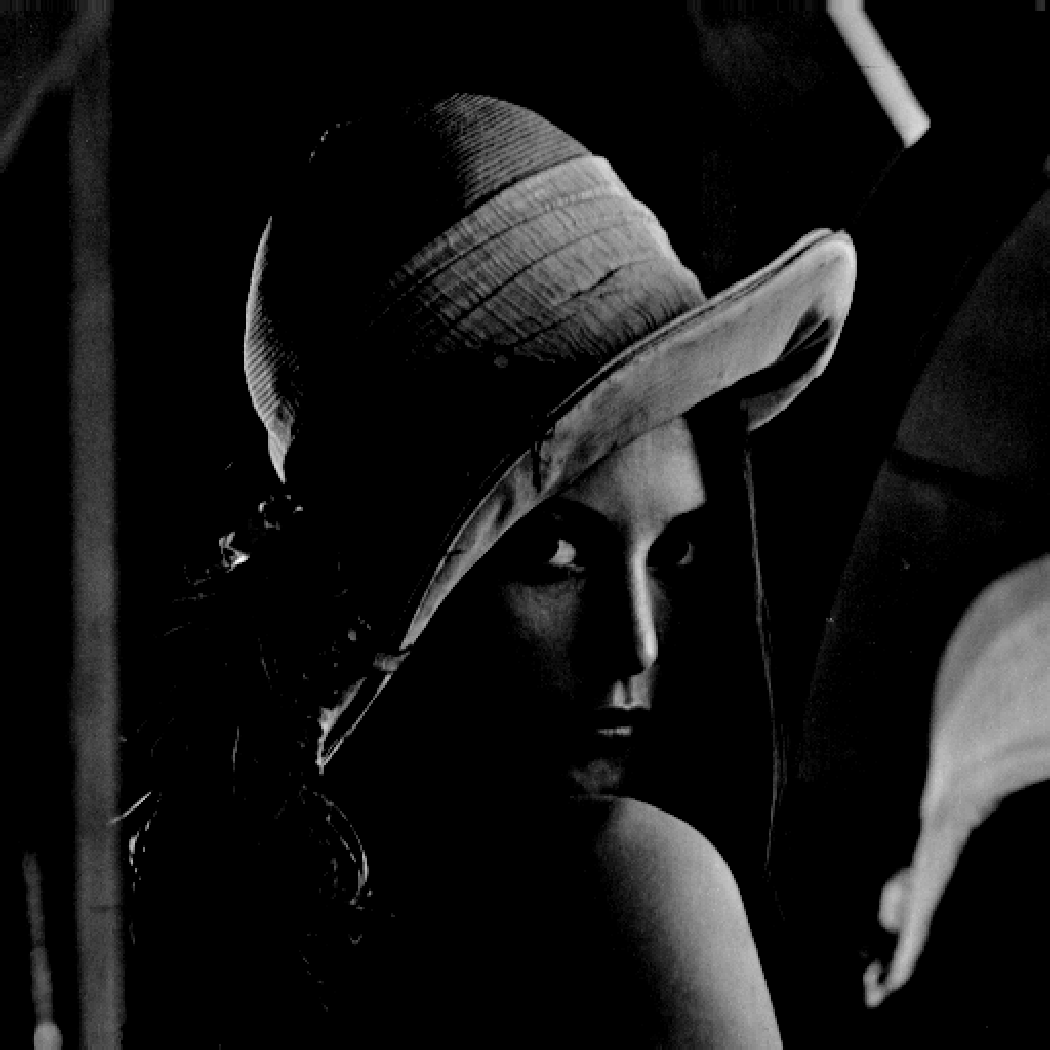
\includegraphics[width=0.5\textwidth]{../imagenes/nivelesLena4.pdf}}
  \subfloat[Imagen reconstruida]{
   \label{f:lenaN4R}
    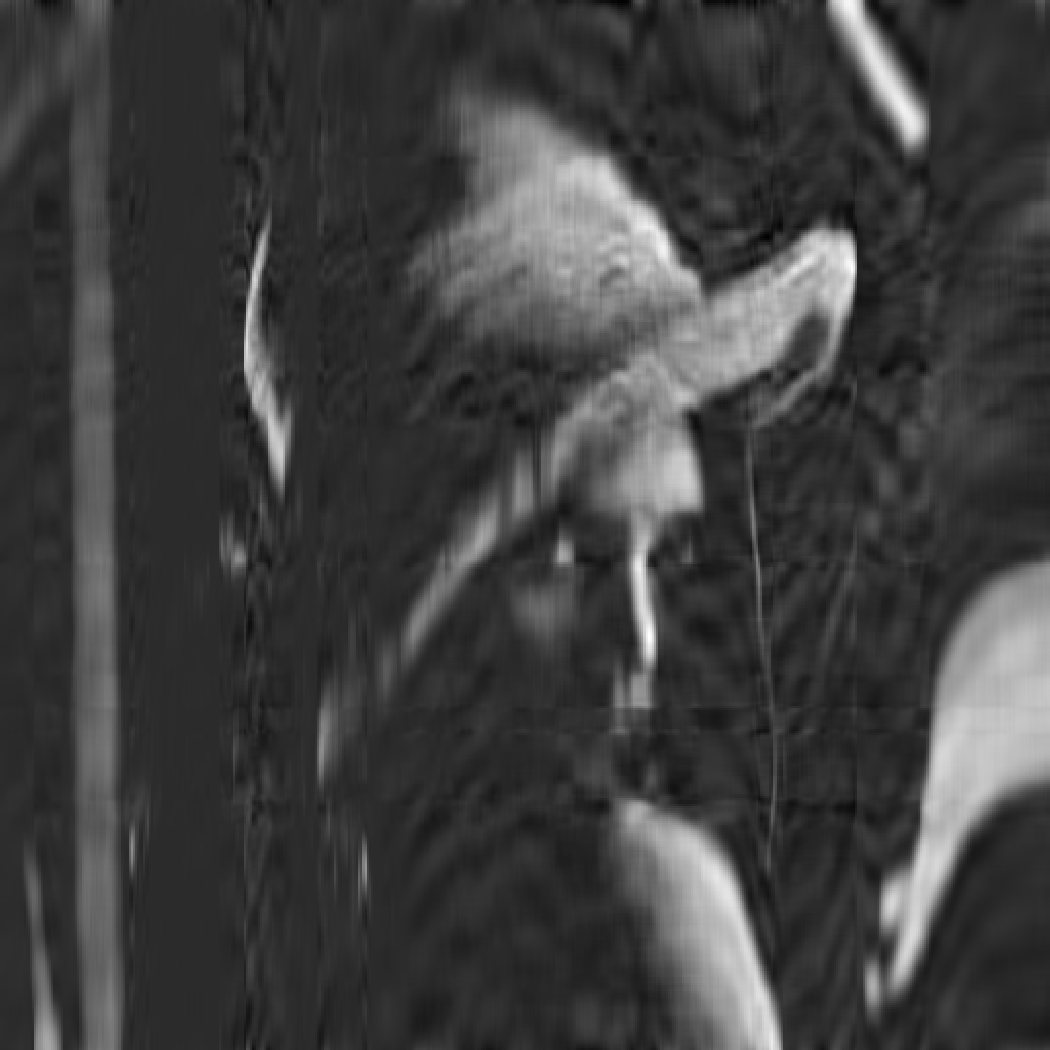
\includegraphics[width=0.5\textwidth]{../imagenes/nivelesLena4r.pdf}}
 \caption{Niveles de Lena}
 \label{f:imgsLenaN4}
\end{figure}

\begin{figure}
 \centering
  \subfloat[Imagen original]{
   \label{f:lenaN5O}
    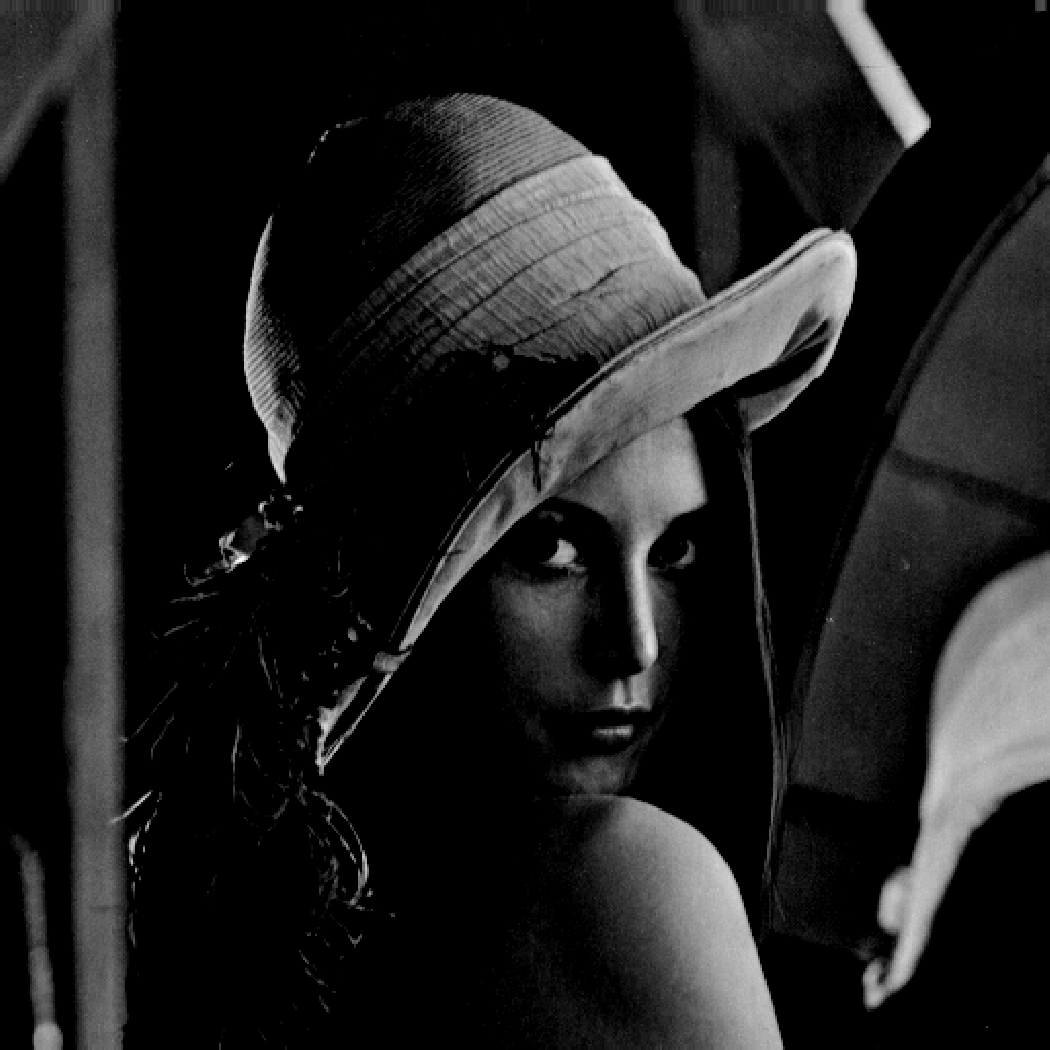
\includegraphics[width=0.5\textwidth]{../imagenes/nivelesLena5.pdf}}
  \subfloat[Imagen reconstruida]{
   \label{f:lenaN5R}
    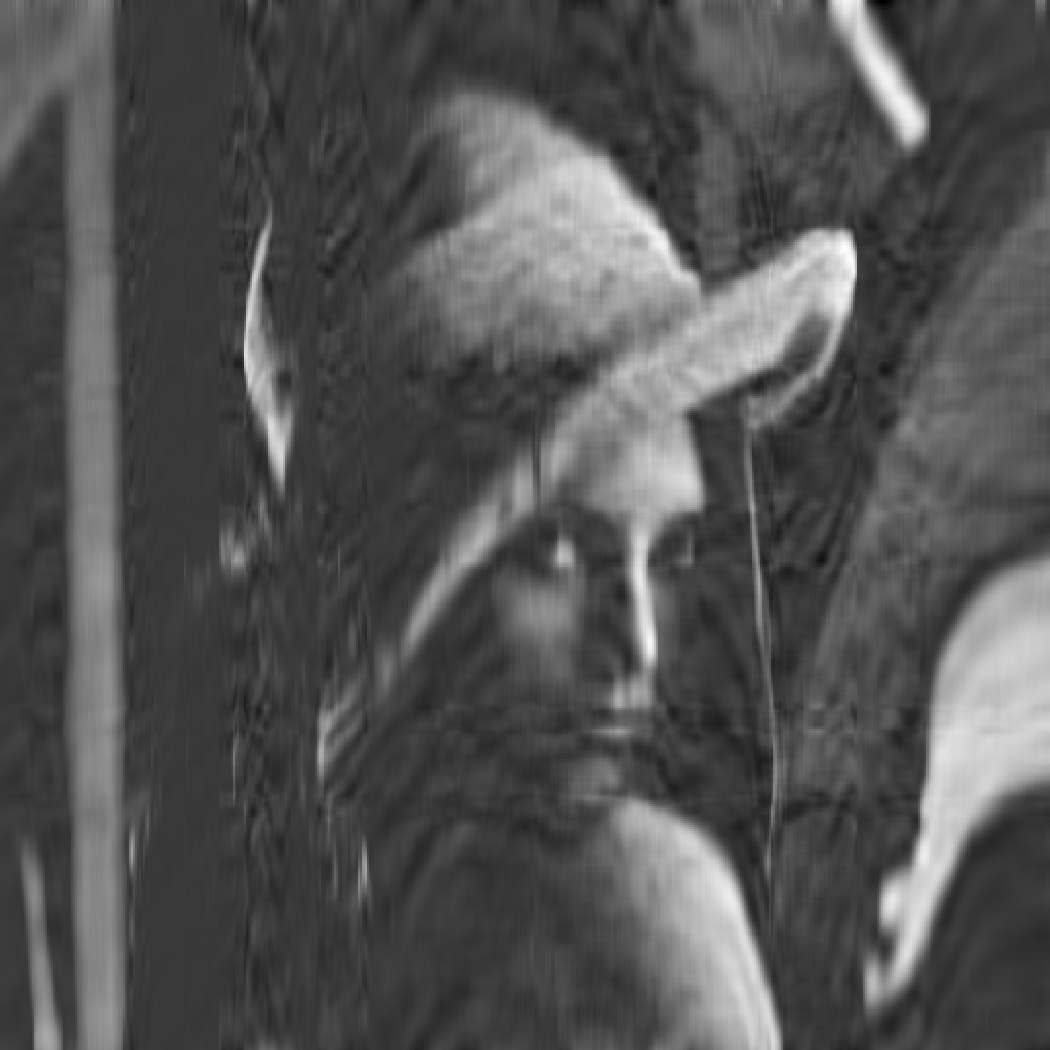
\includegraphics[width=0.5\textwidth]{../imagenes/nivelesLena5r.pdf}}
 \caption{Niveles de Lena}
 \label{f:imgsLenaN5}
\end{figure}

\begin{figure}
 \centering
  \subfloat[Imagen original]{
   \label{f:lenaN6O}
    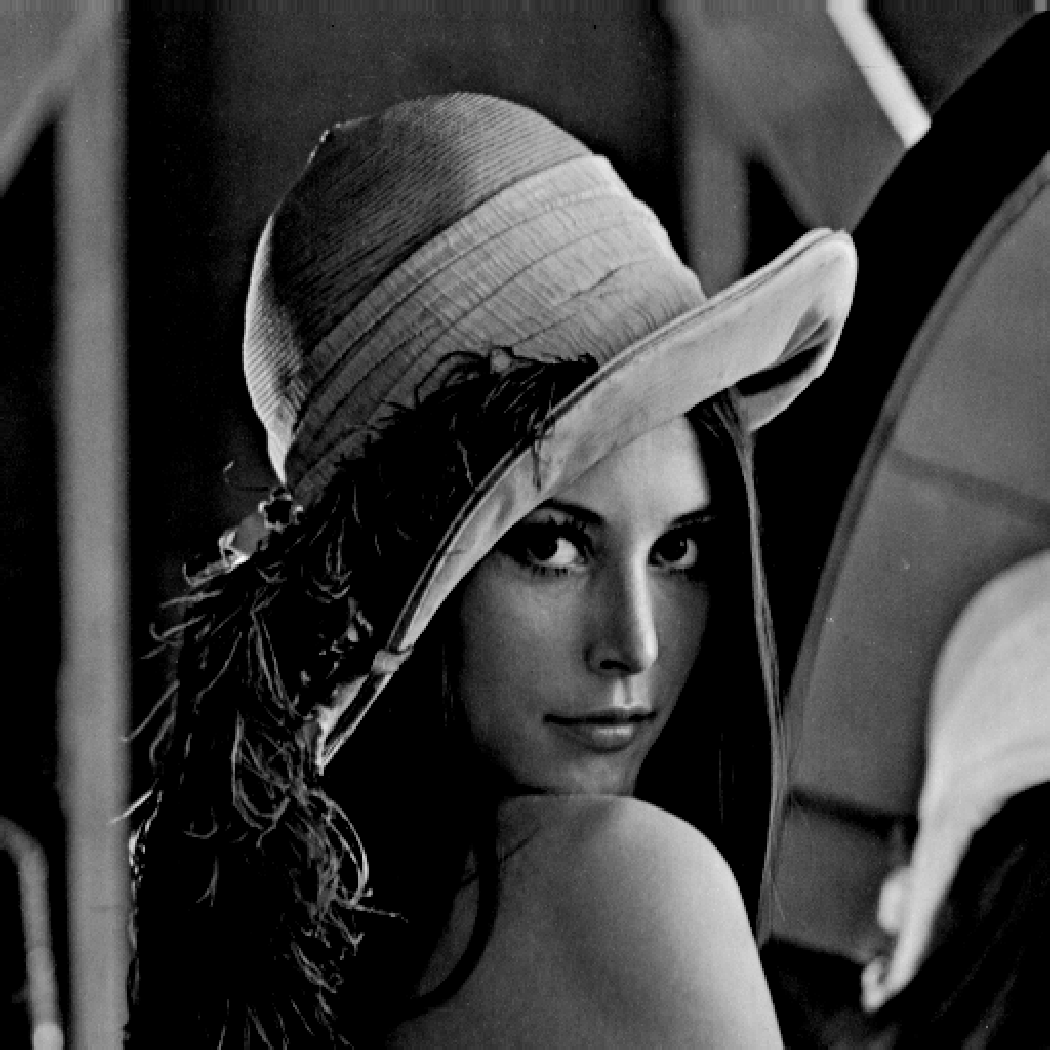
\includegraphics[width=0.5\textwidth]{../imagenes/nivelesLena6.pdf}}
  \subfloat[Imagen reconstruida]{
   \label{f:lenaN6R}
    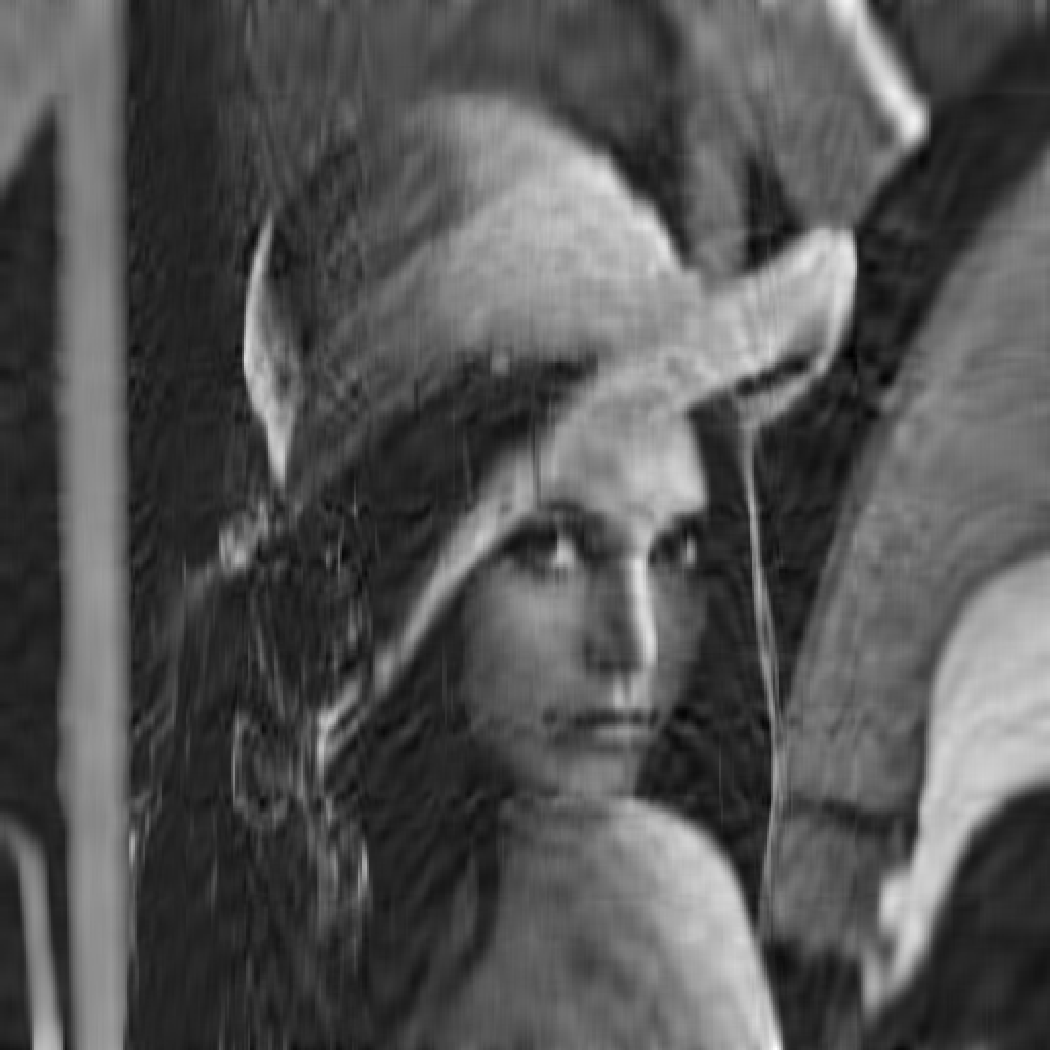
\includegraphics[width=0.5\textwidth]{../imagenes/nivelesLena6r.pdf}}
 \caption{Niveles de Lena}
 \label{f:imgsLenaN6}
\end{figure}

En la figura \ref{f:imgsLenaN2} podemos ver que si la imagen está prácticamente en el mismo color y lo único que aparece en ella tiene mucho contraste, es decir, los cambios en la serie son bruscos, entonces la reconstrucción es bastante buena. Sin embargo en las figuras de la \ref{f:imgsLenaN3} a la \ref{f:imgsLenaN5} vamos viendo como según los cambios son menos bruscos y hay suficiente negro en la imagen, se van viendo peor las reconstrucciones para de nuevo, como podemos ver en la figura \ref{f:imgsLenaN6} y en la original, según van desapareciendo las partes constantes en negro y apareciendo los detalles en distintos tonos (es decir, las series dejan de ser constantes y parecidas) irse viendo con más calidad la imagen reconstruida.\\

Hay que tener en cuenta que para estas reconstrucciones se han sacado componentes principales hasta explicar (como mínimo) el 90\% de varianza y no el 95\%, como estaban hechas las imágenes anteriores. La diferencia entre reconstruir la imagen de Lena original con el 90\% y el 95\% está en la figura \ref{f:imgsLena09}. Es por esto que tampoco se ven con tanta calidad como la imagen reconstruida en la figura \ref{f:lena095}.\\

\begin{figure}
 \centering
  \subfloat[Imagen al 90\%]{
   \label{f:lena090}
    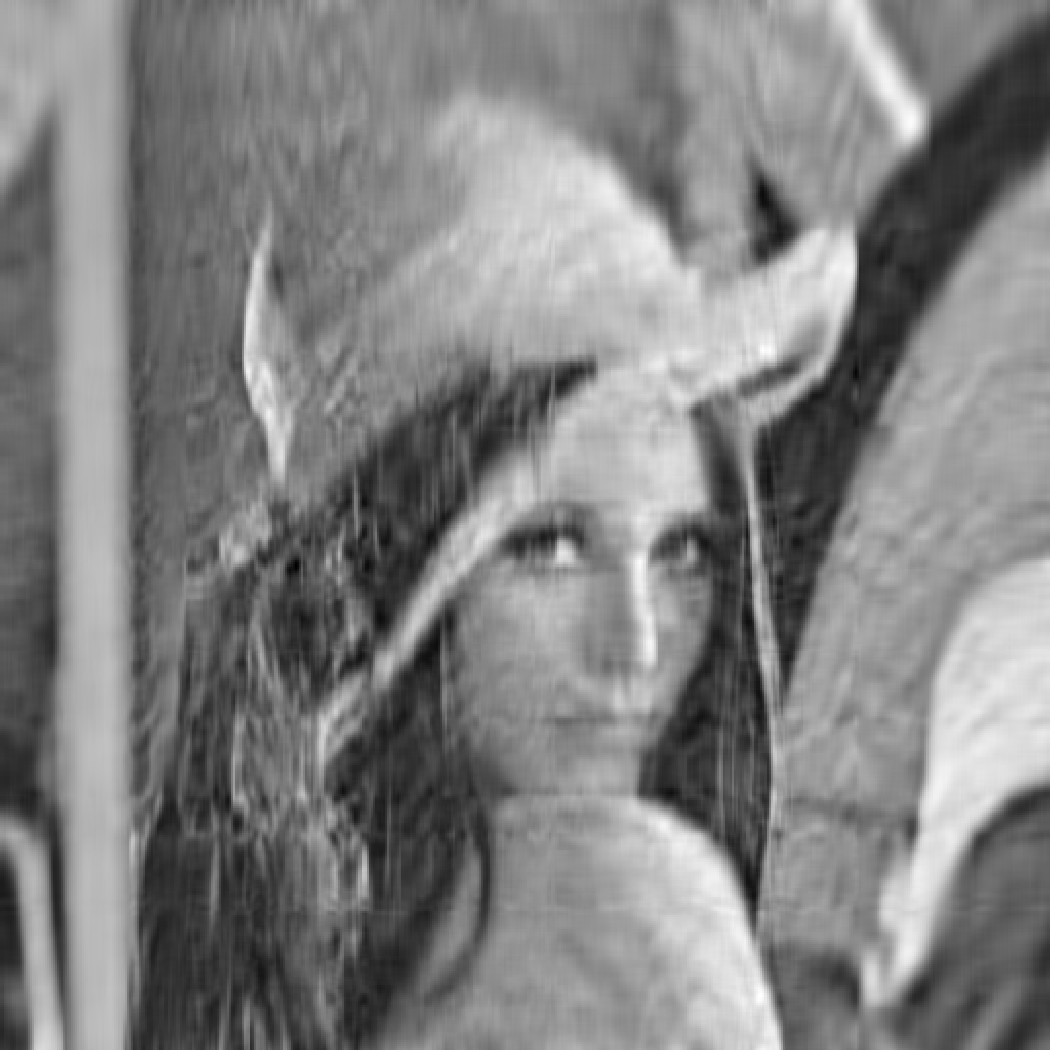
\includegraphics[width=0.5\textwidth]{../imagenes/lena090.pdf}}
  \subfloat[Imagen al 95\%]{
   \label{f:lena095}
    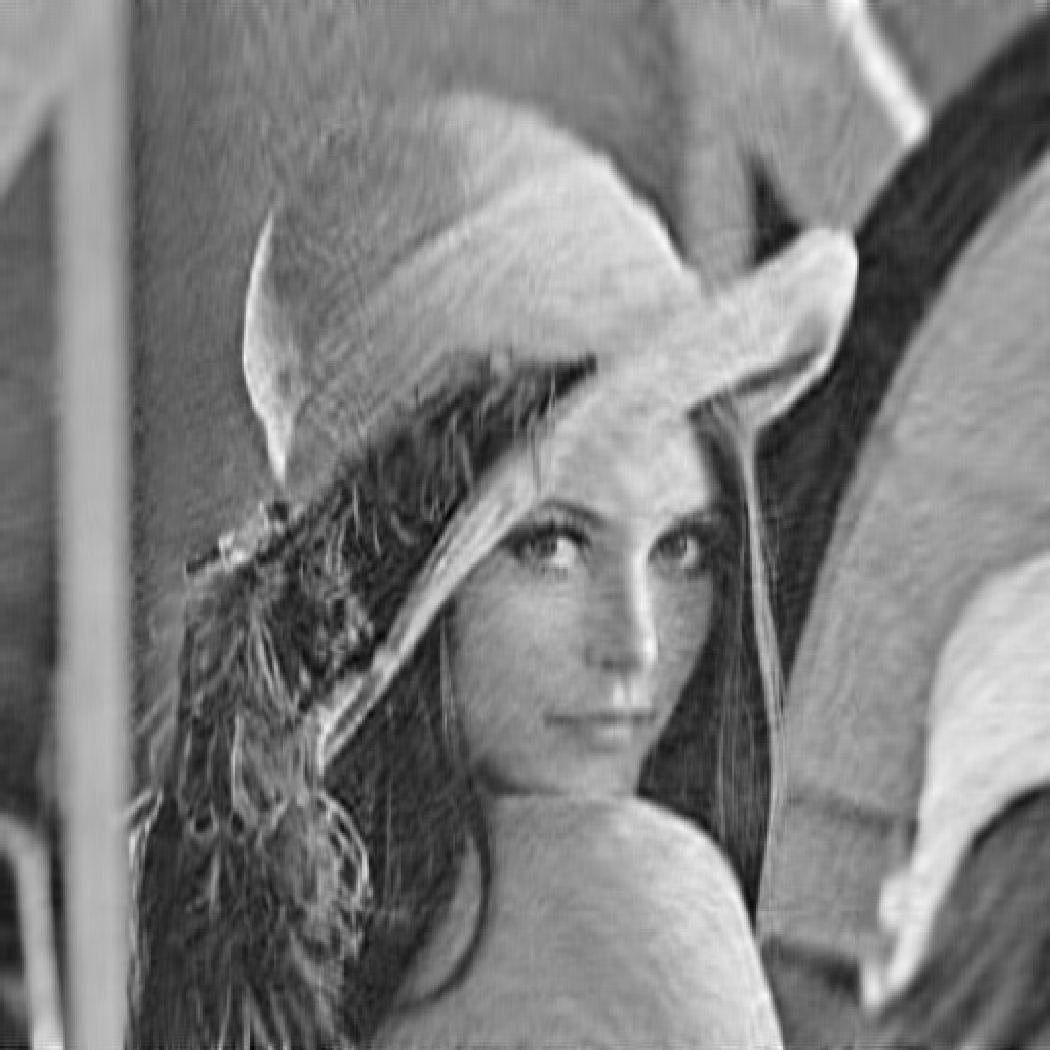
\includegraphics[width=0.5\textwidth]{../imagenes/lena095.pdf}}
 \caption{Reconstrucciones de Lena}
 \label{f:imgsLena09}
\end{figure}

Vamos a ver ahora el factor de compresión que se consigue con cada una de las tres imágenes que hemos utilizado sacando las componentes explicando como mínimo un 95\% de varianza. Esto se puede ver en el cuadro \ref{t:compresion}, donde los cálculos se han hecho de la siguiente forma:
\begin{itemize}
\item El factor de compresión se medirá dividiendo el número de números que son necesarios para almacenar la imagen original entre el número de números necesarios para almacenar lo necesario para reconstruir la imagen, suponiendo que todos los números se almacenan con la misma precisión.
\item En el caso de la imagen original se necesitarán $\text{nº de filas}\times \text{nº de columnas} \times \text{nº de canales}$, ya que se almacena una matriz de píxeles de esas dimensiones.
\item En el caso de las reconstruidas, se almacenan $n$ componentes principales dinámicas y para cada componente principal dinámica de tamaño $T+k$ con $T$ el número de valores en cada serie (el número de filas en este caso) y $k$ el número de lags utilizados en esa componente, se almacena también una matriz de coeficientes $\beta$ de tamaño $m\times (k+1)$, con $m$ el número de series (el número de columnas en este caso) y un vector de coeficientes $\alpha$ de tamaño $m$, por lo que para cada componente se utilizan $(T+k)+m \times (k+1) + m$ y el número total será la suma de estos números para cada componente.
\end{itemize}

\begin{table}[]
\centering
\caption{Factor de compresión}
\label{t:compresion}
\resizebox{\textwidth}{!}{\begin{tabular}{|cc|c|c|c|c|c|c|c|c|}
\hline
                            &         & T   & m   & \begin{tabular}[c]{@{}c@{}}nº\\ componentes\end{tabular} & \begin{tabular}[c]{@{}c@{}}k utilizados\\ (por orden)\end{tabular}                  & nº a almacenar & \begin{tabular}[c]{@{}c@{}}Total en\\ reconstruida\end{tabular} & \begin{tabular}[c]{@{}c@{}}Total en \\ original\end{tabular} & \begin{tabular}[c]{@{}c@{}}Factor de \\ compresión\end{tabular} \\ \hline
Lena                        &         & 512 & 512 & 12                                                       & \begin{tabular}[c]{@{}c@{}}5, 3, 5, 4, 5, 4, \\ 5, 4, 5, 5, 5, 5\end{tabular}       & 46647          & 46647                                                           & 262144                                                       & 5,61974                                                         \\ \hline
\multicolumn{1}{|c|}{}      & Canal R & 546 & 500 & 6                                                        & 4, 4, 5, 4, 5, 5                                                                    & 22803          &                                                                 &                                                              &                                                                 \\ \cline{2-7}
\multicolumn{1}{|c|}{Pato}  & Canal G & 546 & 500 & 5                                                        & 3, 4, 5, 5, 5                                                                       & 18752          & 62855                                                           & 819000                                                       & 13,02999                                                        \\ \cline{2-7}
\multicolumn{1}{|c|}{}      & Canal B & 546 & 500 & 6                                                        & 2, 4, 4, 4, 5, 5                                                                    & 21300          &                                                                 &                                                              &                                                                 \\ \hline
\multicolumn{1}{|c|}{}      & Canal R & 240 & 320 & 10                                                       & \begin{tabular}[c]{@{}c@{}}4, 5, 5, 5, 5, \\ 5, 5, 5, 5, 5\end{tabular}             & 24529          &                                                                 &                                                              &                                                                 \\ \cline{2-7}
\multicolumn{1}{|c|}{Tigre} & Canal G & 240 & 320 & 13                                                       & \begin{tabular}[c]{@{}c@{}}5, 5, 5, 5, 5, \\ 5, 5, 5, 5, 5, \\ 4, 5, 4\end{tabular} & 31663          & 82885                                                           & 230400                                                       & 2,779755                                                        \\ \cline{2-7}
\multicolumn{1}{|c|}{}      & Canal B & 240 & 320 & 11                                                       & \begin{tabular}[c]{@{}c@{}}4, 5, 5, 5, 5, \\ 5, 4, 5, 5, 5, 5\end{tabular}          & 26693          &                                                                 &                                                              &                                                                 \\ \hline
\end{tabular}}
\end{table}

Como vemos en dicha tabla, el factor de compresión depende de cómo de simple sea la imagen, de forma que tenemos que la más simple consigue un factor de compresión de más de 13 y la que tiene más detalles un factor de compresión de casi 3, mientras que Lena, que también tiene bastantes detalles, tiene un factor de compresión de más de 5. Teniendo en cuenta que las componentes principales dinámicas para estas imágenes se han generado exigiendo que se explicara un 95\% de varianza como mínimo, estos factores de compresión son bastante altos, ya que como muy poco se guarda menos de la mitad de la información original.\\


Cabe ahora preguntarse si habría alguna diferencia significativa entre utilizar como series temporales las columnas de la imagen como hemos estado haciendo hasta ahora o utilizar las filas. La intuición nos dice que no debe haber mucha diferencia por lo comentado anteriormente: si un pixel se parece a los que tiene alrededor, tanto las columnas cercanas van a parecerse como series como las filas. Se ha hecho una prueba con la imagen de Lena reconstruida por filas y por columnas y la comparación puede verse en la figura \ref{f:comparativaFilas}.\\

\begin{figure}
 \centering
  \subfloat[Imagen reconstruida por columnas]{
   \label{f:lena095C}
    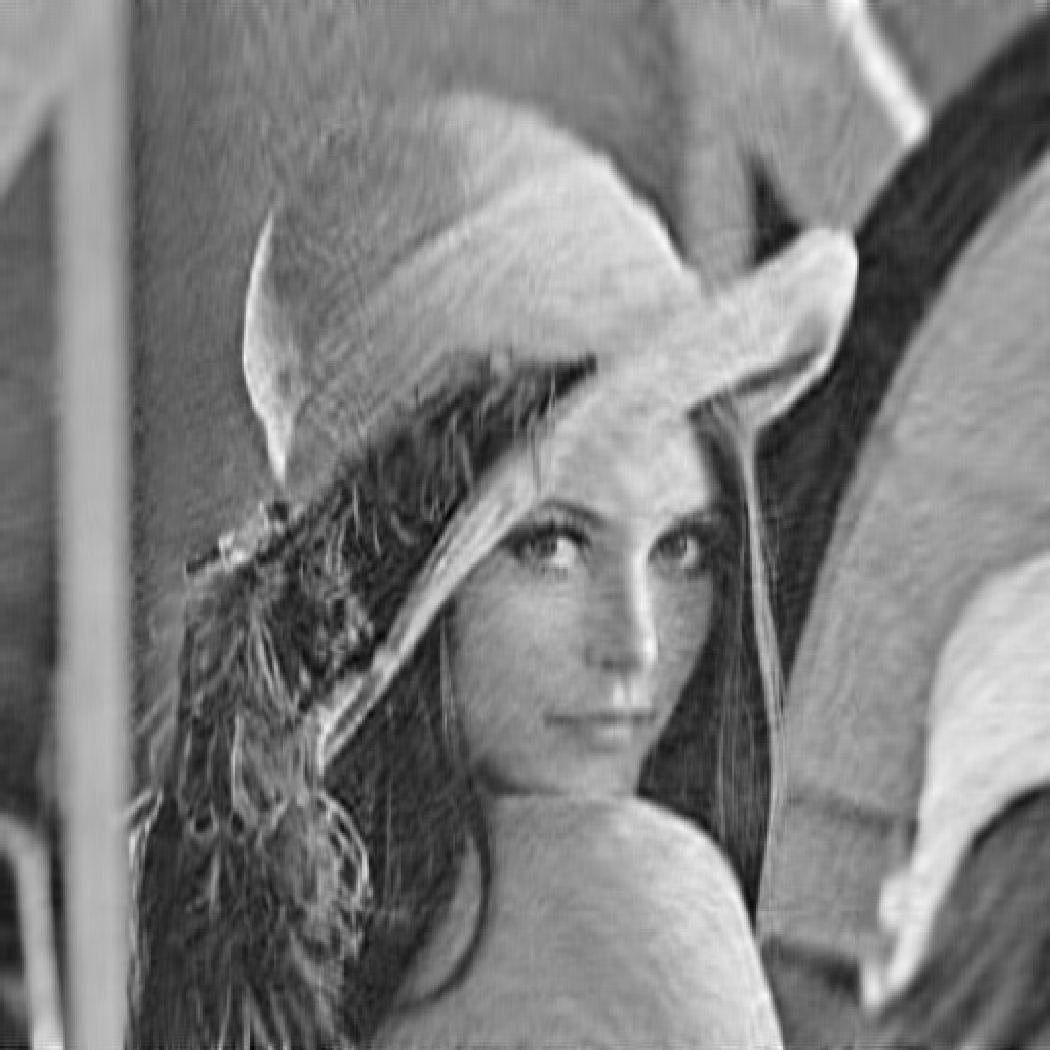
\includegraphics[width=0.5\textwidth]{../imagenes/lena095.pdf}}
  \subfloat[Imagen reconstruida por filas]{
   \label{f:lena095}
    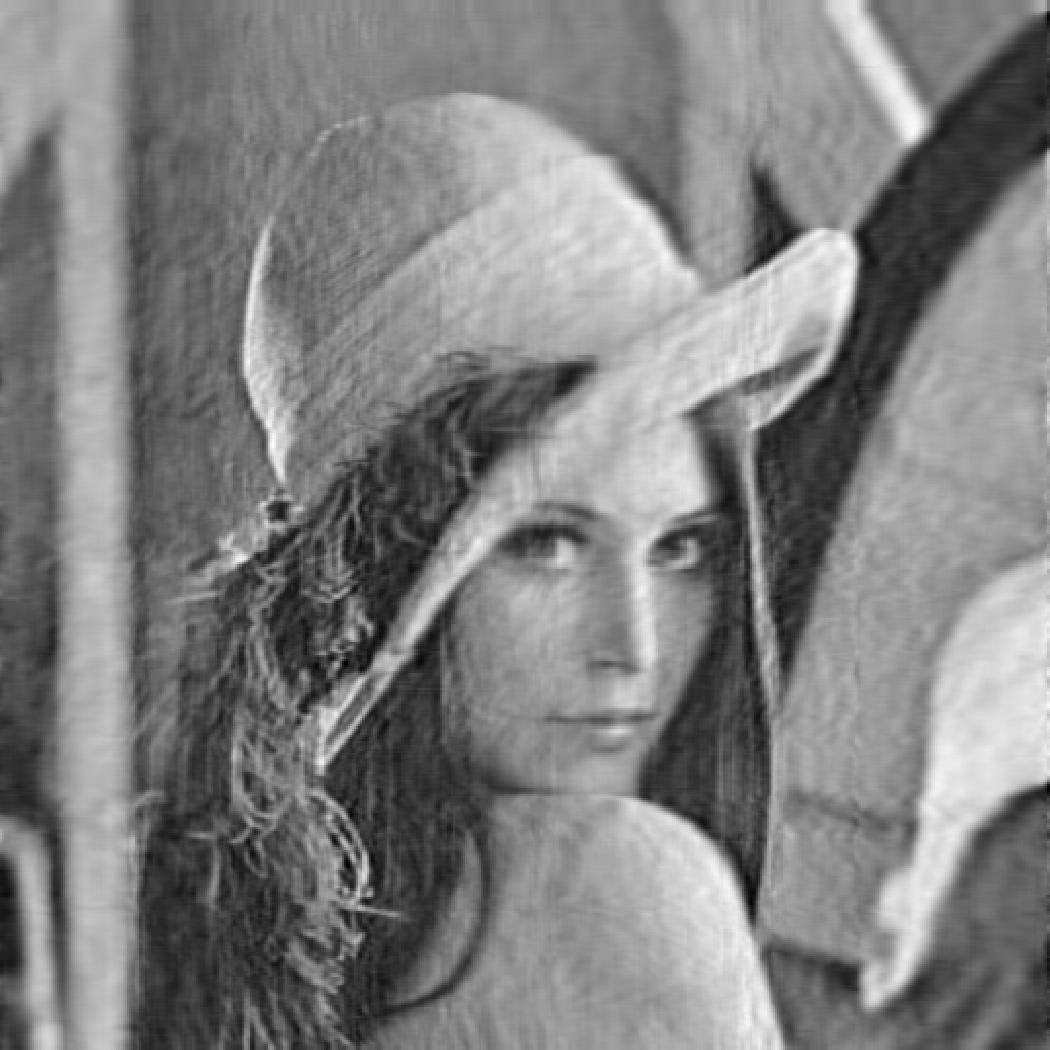
\includegraphics[width=0.5\textwidth]{../imagenes/lenaFilas095.pdf}}
 \caption{Reconstrucciones de Lena}
 \label{f:comparativaFilas}
\end{figure}

Efectivamente, las diferencias no son significativas. Sí que podemos observar que hay partes más nítidas en una que en otra. Por ejemplo, los ojos están más nítidos en la imagen reconstruida por columnas y la parte superior del sombrero está más nítida en la imagen reconstruida por filas.\\

Como último experimento dentro de la compresión de imágenes se ha elegido ver las reconstrucciones con sucesivas componentes principales dinámicas, acumulándolas, para ver el efecto que éstas tienen en la reconstrucción de las series originales. Es decir, hemos cogido la imagen de Lena y la hemos reconstruido sólo con la primera componente, después con la primera y la segunda, etcétera, hasta llegar a las 12 componentes que obtiene el método \texttt{auto.gdpc}. El resultado de estos experimentos se puede ver en las figuras \ref{f:RLenaC1}, \ref{f:RLenaC2}, \ref{f:RLenaC3} y \ref{f:RLenaC4}.

\begin{figure}[]
 \centering
  \subfloat[Componente 1]{
   \label{f:lena0951}
    \includegraphics[width=0.33\textwidth]{../imagenes/lena0951.pdf}}
  \subfloat[Componentes 1 y 2]{
   \label{f:lena0952}
    \includegraphics[width=0.33\textwidth]{../imagenes/lena0952.pdf}}
  \subfloat[Componentes 1, 2 y 3]{
   \label{f:lena0953}
    \includegraphics[width=0.33\textwidth]{../imagenes/lena0953.pdf}}
 \caption{Reconstrucciones de Lena con distintas componentes}
 \label{f:RLenaC1}
\end{figure}

\begin{figure}[]
 \centering
  \subfloat[Componentes 1 a 4]{
   \label{f:lena0954}
    \includegraphics[width=0.33\textwidth]{../imagenes/lena0954.pdf}}
  \subfloat[Componentes 1 a 5]{
   \label{f:lena0955}
    \includegraphics[width=0.33\textwidth]{../imagenes/lena0955.pdf}}
  \subfloat[Componentes 1 a 6]{
   \label{f:lena0956}
    \includegraphics[width=0.33\textwidth]{../imagenes/lena0956.pdf}}
 \caption{Reconstrucciones de Lena con distintas componentes}
 \label{f:RLenaC2}
\end{figure}


\begin{figure}[]
 \centering
  \subfloat[Componentes 1 a 7]{
   \label{f:lena0957}
    \includegraphics[width=0.33\textwidth]{../imagenes/lena0957.pdf}}
  \subfloat[Componentes 1 a 8]{
   \label{f:lena0958}
    \includegraphics[width=0.33\textwidth]{../imagenes/lena0958.pdf}}
  \subfloat[Componentes 1 a 9]{
   \label{f:lena0959}
    \includegraphics[width=0.33\textwidth]{../imagenes/lena0959.pdf}}
 \caption{Reconstrucciones de Lena con distintas componentes}
 \label{f:RLenaC3}
\end{figure}

\begin{figure}[]
 \centering
  \subfloat[Componentes 1 a 10]{
   \label{f:lena09510}
    \includegraphics[width=0.33\textwidth]{../imagenes/lena09510.pdf}}
  \subfloat[Componentes 1 a 11]{
   \label{f:lena09511}
    \includegraphics[width=0.33\textwidth]{../imagenes/lena09511.pdf}}
  \subfloat[Componentes 1 a 12]{
   \label{f:lena09512}
    \includegraphics[width=0.33\textwidth]{../imagenes/lena09512.pdf}}
 \caption{Reconstrucciones de Lena con distintas componentes}
 \label{f:RLenaC4}
\end{figure}

Como se puede observar, la mejora de la reconstrucción conforme se van agregando componentes hasta la octava es obvia, ya que se pasa de ver una simple silueta a ver la imagen original. Agregar la información que aportan el resto de componentes le da a la reconstrucción la nitidez que veíamos al principio. Esto es así porque la información que va aportando cada componente se suma a la que información de la que ya se disponía, como se ha comentado antes.\\ %TODO

%TODO conclusiones en la utilización a compresión de imágenes en general

\section{Aplicación: Búsqueda de patrones en series periódicas}

Una de las técnicas en el preprocesamiento de series es eliminar los periodos de las series originales, ya que es uno de los pasos para hacerlas estacionarias, en caso de que éstas sean periódicas. Se ha pensado en utilizar el algoritmo GDPC para obtener el patrón periódico de la serie y restárselo directamente a la serie original por periodos. Para ello, se toma la serie original y se divide en periodos y se coloca cada trozo de la serie original como una columna de una matriz, sobre la que se pasará el GDPC. Al ser las series parecidas, lo más probable es que sólo se obtenga una componente principal dinámica, de modo que ésta será la que utilicemos. En caso de que se obtenga más de una, siempre se puede aumentar \texttt{k\_max} o disminuir un poco \texttt{expl\_var} en el algoritmo para obtener una sola componente principal dinámica.\\

Para probar si de hecho se pueden utilizar las componentes principales dinámicas para la detección de patrones o no, se ha hecho un experimento con una serie real que tiene una tendencia periódica. Esta serie es la cantidad de accidentes de coche mensuales en Italia desde enero de 1983 hasta diciembre de 1997, obtenida de la referencia %TODO
y que se puede ver en la figura \ref{f:accidents}. Como se puede ver esta serie presenta una clara tendencia periódica, lo que tiene sentido porque hay más accidentes en verano que en invierno.

\begin{figure}[]
 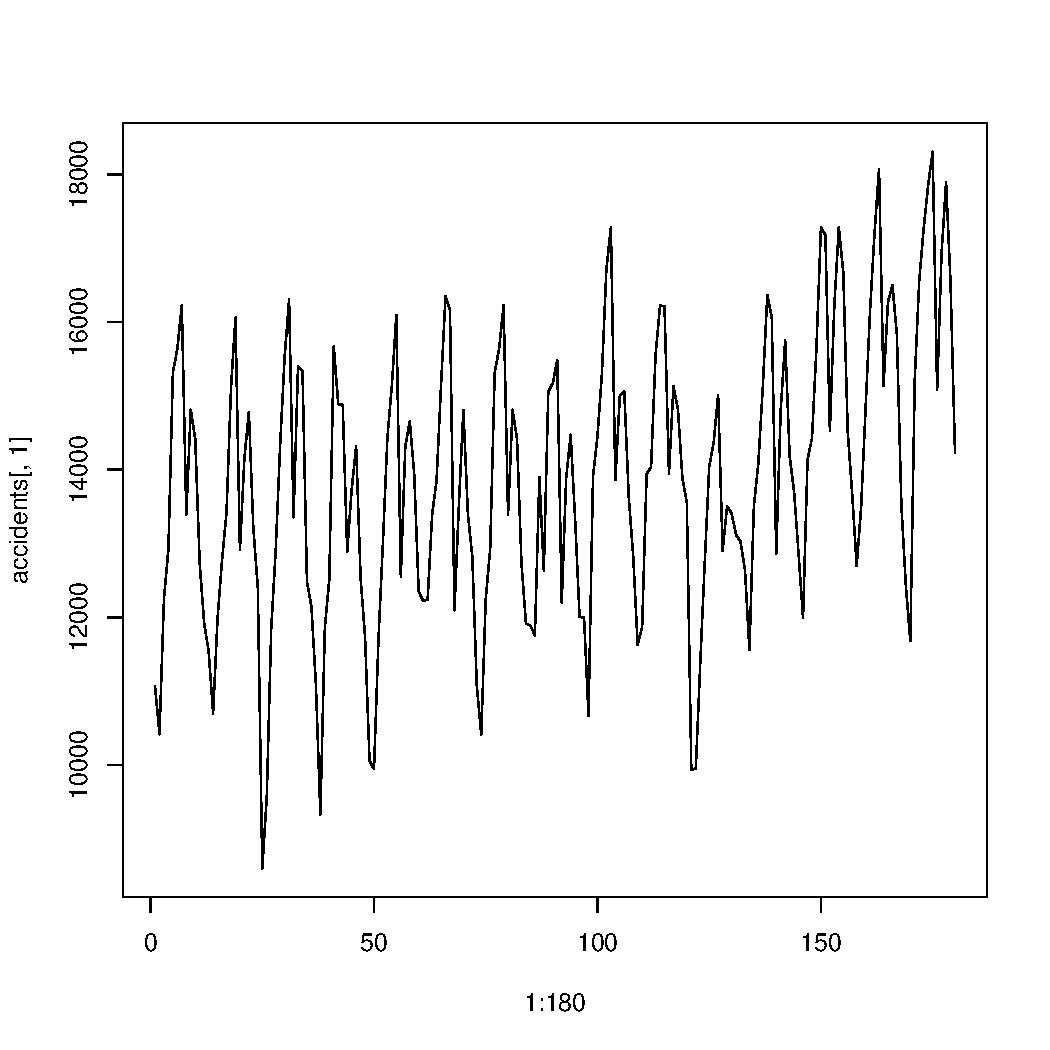
\includegraphics[width=\textwidth, height=0.4\textheight]{../imagenes/accidents.pdf}
 \caption{Número mensual de accidentes de coche en Italia de 1983 a 1997}
 \label{f:accidents}
\end{figure}

Lo que hacemos ahora es cortar trozos de esta serie de la forma en la que aparece en la figura \ref{f:periodos} de forma que cada serie consta de 13 puntos, y los metemos todos en una matriz, por columnas, para obtener la primera componente principal. En este caso se consigue sólo una imponiendo en el algoritmo \texttt{k\_max=5} y \texttt{expl\_var=0.95}. El resultado de esta componente está en la figura \ref{f:accidentsComp}.

\begin{figure}[]
 \centering
  \subfloat[Primer periodo]{
   \label{f:periodo1}
    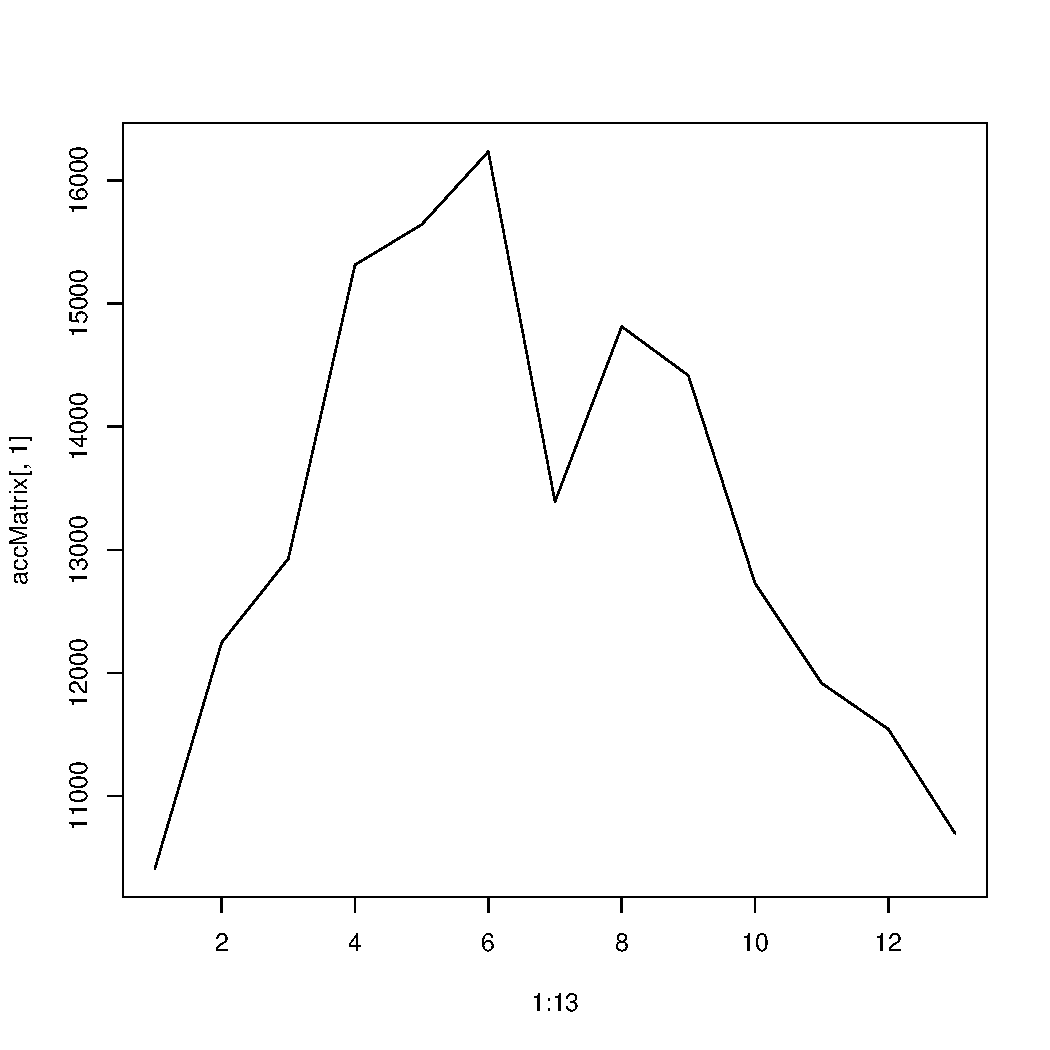
\includegraphics[width=0.33\textwidth]{../imagenes/primerPeriodo.pdf}}
  \subfloat[Segundo periodo]{
   \label{f:periodo2}
    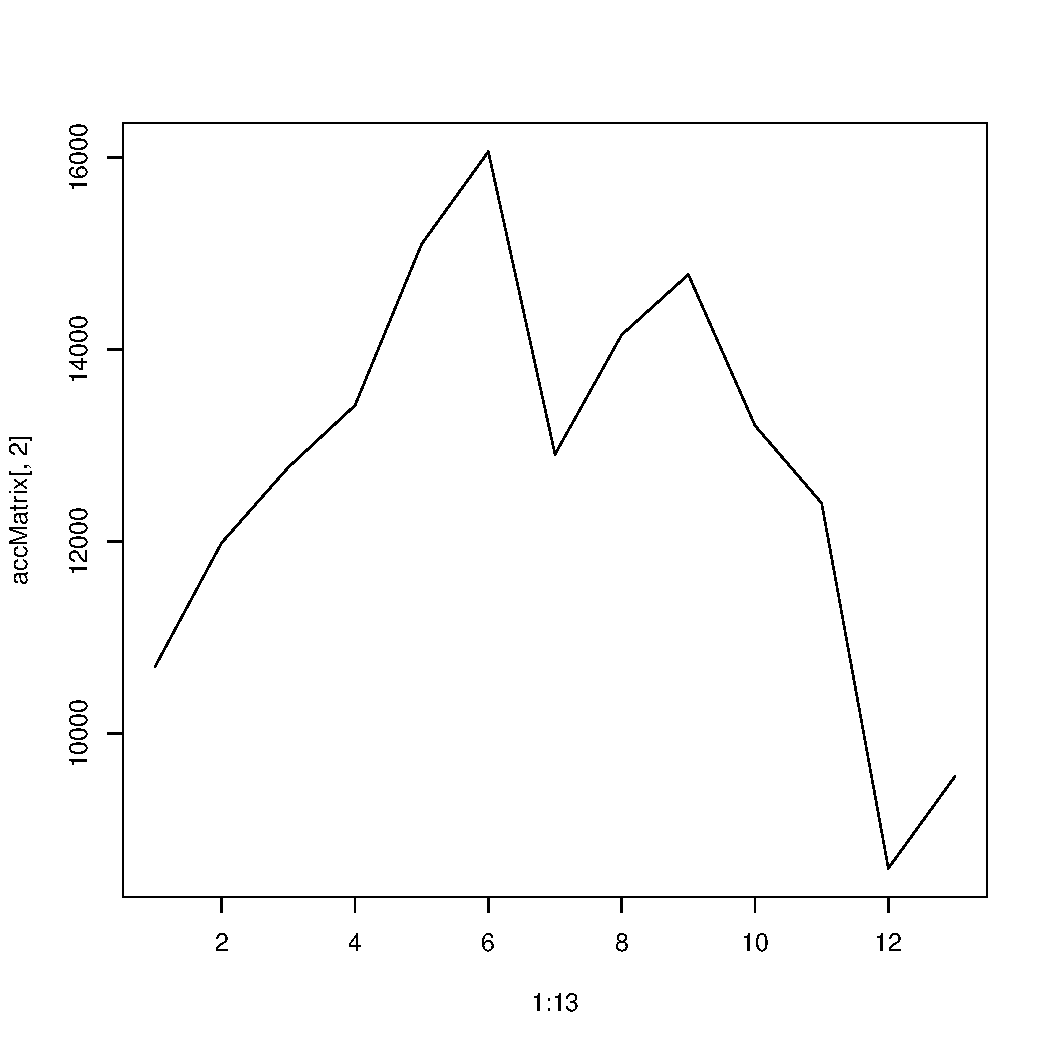
\includegraphics[width=0.33\textwidth]{../imagenes/segundoPeriodo.pdf}}
  \subfloat[Tercer periodo]{
   \label{f:periodo3}
    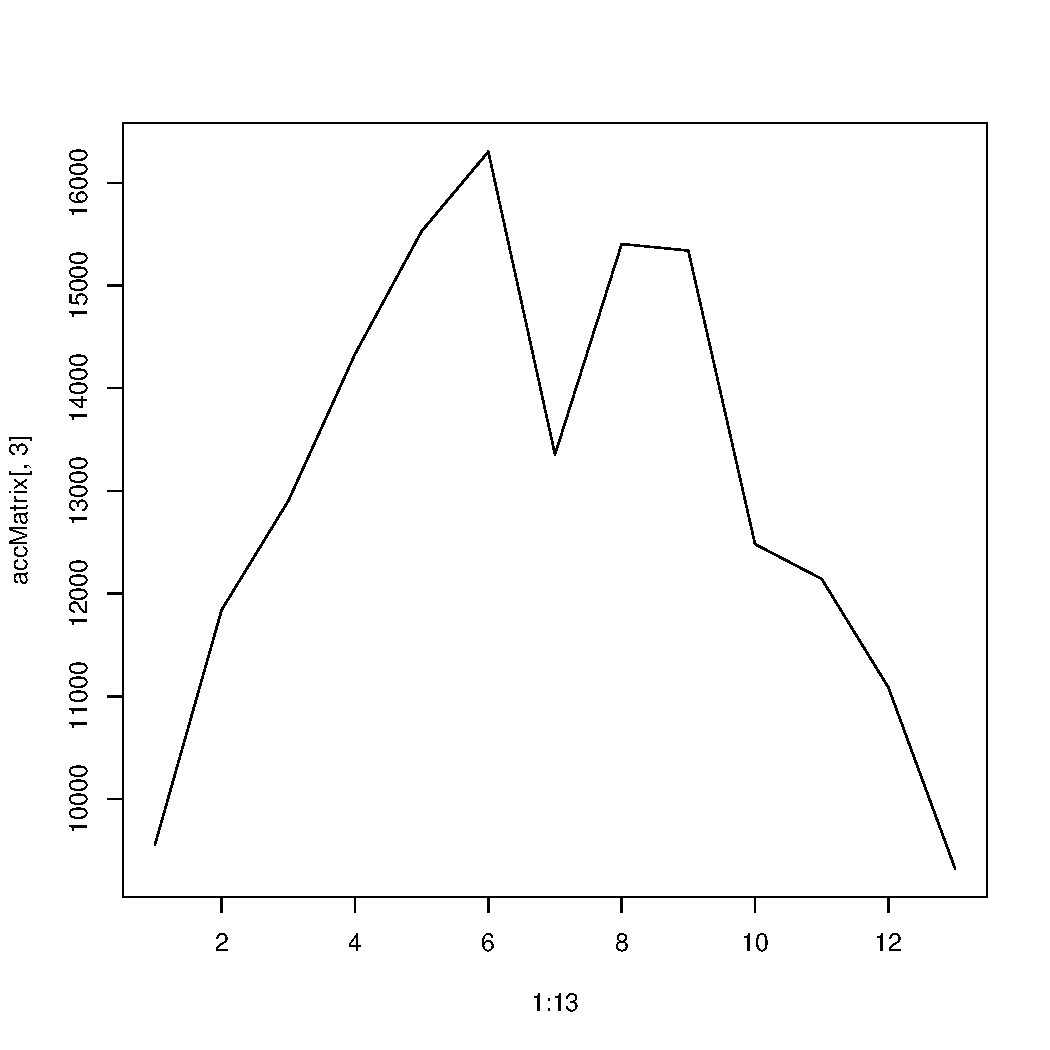
\includegraphics[width=0.33\textwidth]{../imagenes/tercerPeriodo.pdf}}
 \caption{Primeros periodos de la serie de accidentes en Italia}
 \label{f:periodos}
\end{figure}

\begin{figure}[]
 \centering
 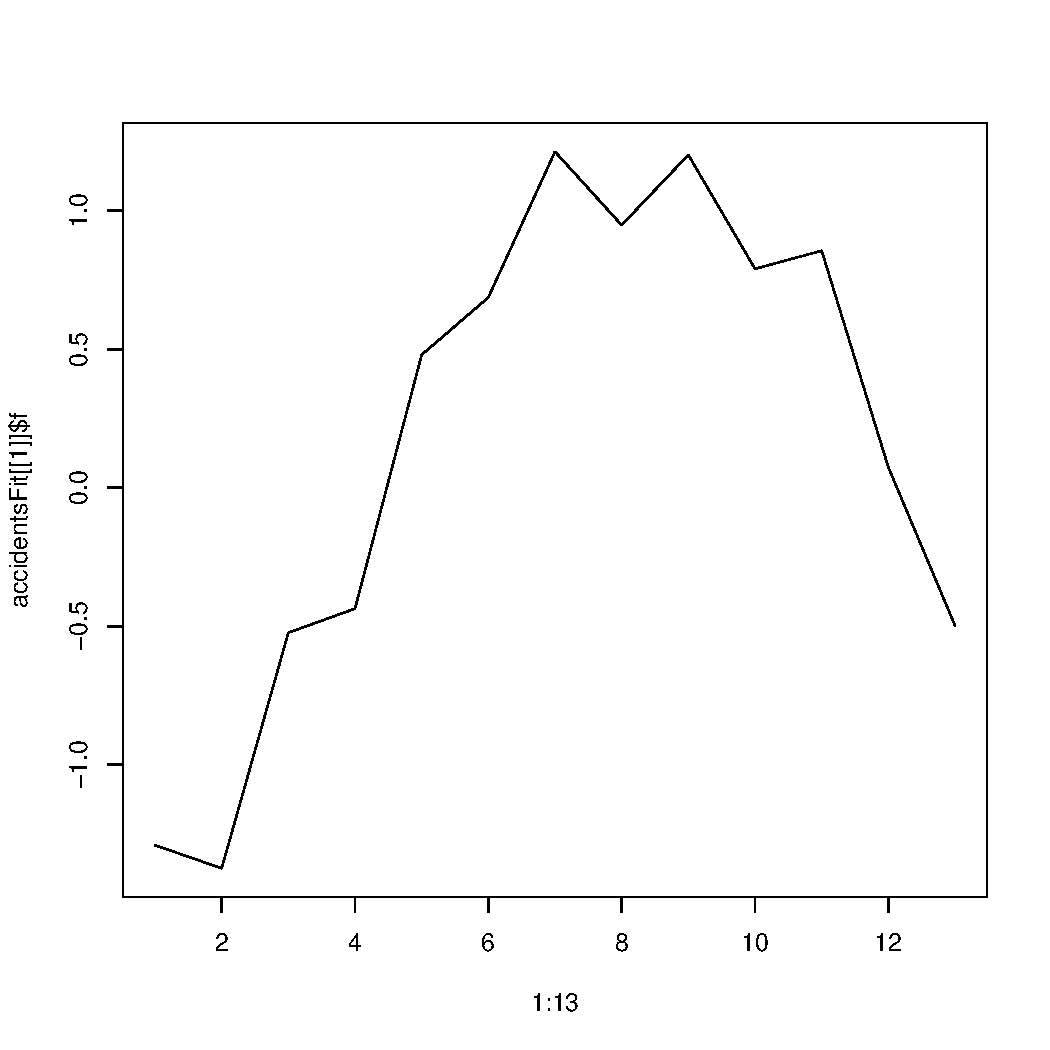
\includegraphics[width=0.5\textwidth]{../imagenes/accidentsComp.pdf}
 \caption{Componente principal dinámica para la serie de accidentes}
 \label{f:accidentsComp}
\end{figure}

En la figura \ref{f:accidentsComp} obtenemos por tanto un "patrón" del periodo de la serie original. Este patrón se obtiene en el intervalo $[-1, 1]$ y los valores de la serie original son mucho mayores, como se puede ver en la figura \ref{f:accidents}. Por esto, para restarle este patrón a la serie original se ha multiplicado el mismo, en cada intervalo periódico, por la media de la serie original en ese intervalo periódico antes de restarlo. El resultado se puede ver en la figura \ref{f:accidentsSinPatron}.

\begin{figure}[]
 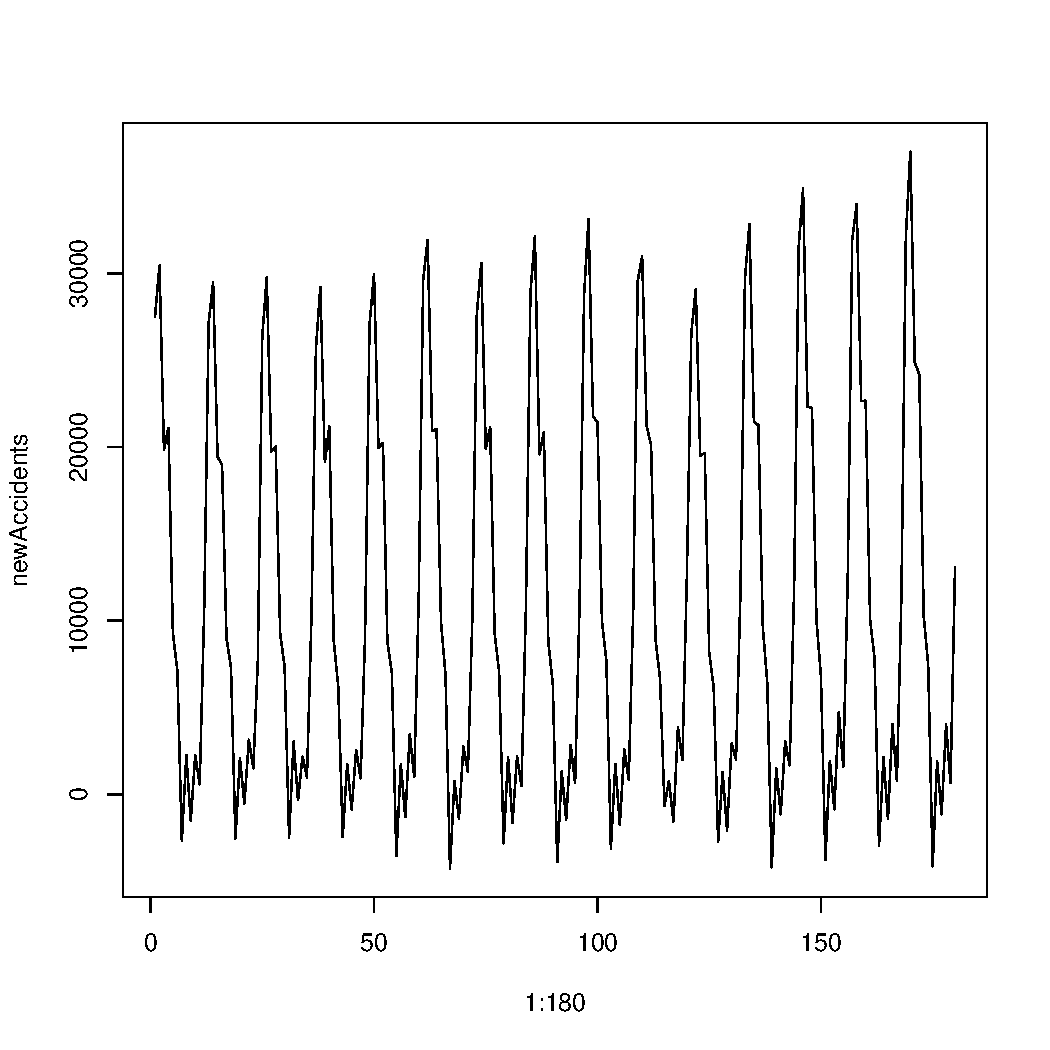
\includegraphics[width=\textwidth, height=0.4\textheight]{../imagenes/accidentsSinPatron.pdf}
 \caption{Serie de accidentes de coche en Italia sin patrón}
 \label{f:accidentsSinPatron}
\end{figure}

%TODO esto es así?


\section{Aplicación: Predicción de un conjunto de series temporales}

Como última aplicación, y quizás la más importante de todas las que hemos visto, vamos a ver si es posible predecir valores de un conjunto de series temporales a través de las componentes principales y las matrices de coeficientes $\beta$ y $\alpha$ que se obtienen con el método GDPC. La idea es la siguiente: supongamos que tenemos un conjunto de 100 series temporales, midiendo una información similar (por ejemplo, número de accidentes de coche mensuales en diferentes países) de los que queremos predecir los 5 siguientes valores de cada una de ellas. En lugar de tomar cada serie por separado y predecir sus siguientes 5 valores, vamos a obtener las componentes principales dinámicas, junto con sus coeficientes, y vamos a tratar cada componente principal como una nueva serie a la que le vamos a predecir sus próximos 5 valores. El número de componentes principales obtenidas será mucho menor que el número de series originales, por lo que el trabajo de predicción de nuevos valores será también mucho menor. Una vez tenemos los valores predichos de las componentes principales volvemos hacia atrás reconstruyendo los valores originales más los valores predichos con los coeficientes que habíamos sacado inicialmente con el método GDPC. Esto se puede hacer porque en la reconstrucción el único parámetro que depende de $T$, el número de valores en cada serie, es $\mathbf{f}$. Vamos a ver un pequeño ejemplo para verlo mejor. Recordemos que la reconstrucción con $k$ leads (que es equivalente a tener lags), $1 \leq j \leq m$, $1 \leq t \leq T$, está dada por
\begin{equation}\label{eq:recons}
	\widehat{z}_{j,t} = \sum_{i=0}^k \beta_{j,i+1}f_{t-i} + \alpha_j.
\end{equation}

Supongamos que inicialmente tenemos $m=3$ series de $T=5$ valores cada una y que obtenemos una única componente principal $\mathbf{f}$ obtenida con $k=4$ leads y que por tanto tendrá una longitud de $5+4=9$ valores, $\mathbf{f} = (f_1, f_2, \dots, f_9)$. Supongamos que queremos obtener los dos siguientes valores de las 3 series y para ello lo que hacemos es predecir los dos siguientes valores de $\mathbf{f}$, a los que vamos a llamar $\widehat{f}_{10}$ y $\widehat{f}_{11}$. Entonces definimos una extensión de $\mathbf{f}$, $\mathbf{\widehat{f}}$ como $\mathbf{\widehat{f}} = (f_1, \dots, f_9, \widehat{f}_{10}, \widehat{f}_{11})$ y vamos a realizar la reconstrucción dada por (\ref{eq:recons}) utilizando $\mathbf{\widehat{f}}$ en lugar de $\mathbf{f}$.\\

Entonces, si queremos reconstruir alguno de los valores originales de las series, no cambia nada. Por ejemplo, supongamos que queremos reconstruir $\widehat{z}_{3,5}$, entonces tenemos que,
\[	\widehat{z}_{3,5} = \beta_{3,1}f_5 + \beta_{3,2}f_6 + \beta_{3,3}f_7 + \beta_{3,4}f_8 + \beta_{3,5}f_9 + \alpha_3	\]

Ahora, podemos obtener también los valores $\widehat{z}_{1,6}$, $\widehat{z}_{2,6}$, $\widehat{z}_{3,6}$, $\widehat{z}_{1,7}$, $\widehat{z}_{2,7}$, $\widehat{z}_{3,7}$, que no estaban en las series originales, mediante las expresiones
\[	\widehat{z}_{1,6} = \beta_{1,1}f_6 + \beta_{1,2}f_7 + \beta_{1,3}f_8 + \beta_{1,4}f_9 + \beta_{1,5}\widehat{f}_{10} + \alpha_1	\]
\[	\widehat{z}_{2,6} = \beta_{2,1}f_6 + \beta_{2,2}f_7 + \beta_{2,3}f_8 + \beta_{2,4}f_9 + \beta_{2,5}\widehat{f}_{10} + \alpha_2	\]
\[	\widehat{z}_{3,6} = \beta_{3,1}f_6 + \beta_{3,2}f_7 + \beta_{3,3}f_8 + \beta_{3,4}f_9 + \beta_{3,5}\widehat{f}_{10} + \alpha_3	\]
\[	\widehat{z}_{1,7} = \beta_{1,1}f_7 + \beta_{1,2}f_8 + \beta_{1,3}f_9 + \beta_{1,4}\widehat{f}_{10} + \beta_{1,5}\widehat{f}_{11} + \alpha_1	\]
\[	\widehat{z}_{2,7} = \beta_{2,1}f_7 + \beta_{2,2}f_8 + \beta_{2,3}f_9 + \beta_{2,4}\widehat{f}_{10} + \beta_{2,5}\widehat{f}_{11} + \alpha_2	\]
\[	\widehat{z}_{3,7} = \beta_{3,1}f_7 + \beta_{3,2}f_8 + \beta_{3,3}f_9 + \beta_{3,4}\widehat{f}_{10} + \beta_{3,5}\widehat{f}_{11} + \alpha_3	\]

Esto tiene un inconveniente y es que a más valores intentemos predecir de $\mathbf{f}$ peor serán los valores obtenidos al hacer la reconstrucción porque los coeficientes, tanto los $\beta_{j,t}$ como los $\alpha_j$ se han generado con los valores conocidos de las series $z_{j,t}$ y no tienen por qué funcionar también para los valores predichos de $\mathbf{f}$. Sin embargo, este es un problema presente siempre que se trata la predicción de series temporales: a mayor horizonte de predicción, menos fiables son los resultados.\\

Para probar esto experimentalmente se han hecho un par de pruebas con el conjunto de datos \texttt{ipi91} disponible en el paquete \texttt{gdpc}. Concretamente, con las 4 primeras series, y utilizando 12 valores menos de los disponibles en cada serie para la obtención de las componentes principales dinámicas, para tener con qué comparar los valores predichos.

Se han cogido por tanto las series del IPI (Industrial Production Index) de Francia, Alemania, Italia y Reino Unido de los valores 1 al 252, se han metido en una matriz, por columnas, y se ha obtenido, con \texttt{k\_max = 10} y \texttt{expl\_var=0.95} una componente principal. Esta componente principal se ha modelado con un modelo AR(2) y con un modelo ARMA(2,2), obteniendo con cada uno de ellos los 5 siguientes valores. Después se ha hecho la reconstrucción de las series originales con los valores devueltos con el modelo AR(2) y los valores devueltos con el modelo ARMA(2,2) y en las figuras \ref{f:francia}, \ref{f:alemania}, \ref{f:italia} y \ref{f:uk} se pueden ver los últimos 100 valores de cada serie (incluyendo los 5 predichos).

\begin{figure}[]
 \centering
  \subfloat[Serie original]{
   \label{f:franciaO}
    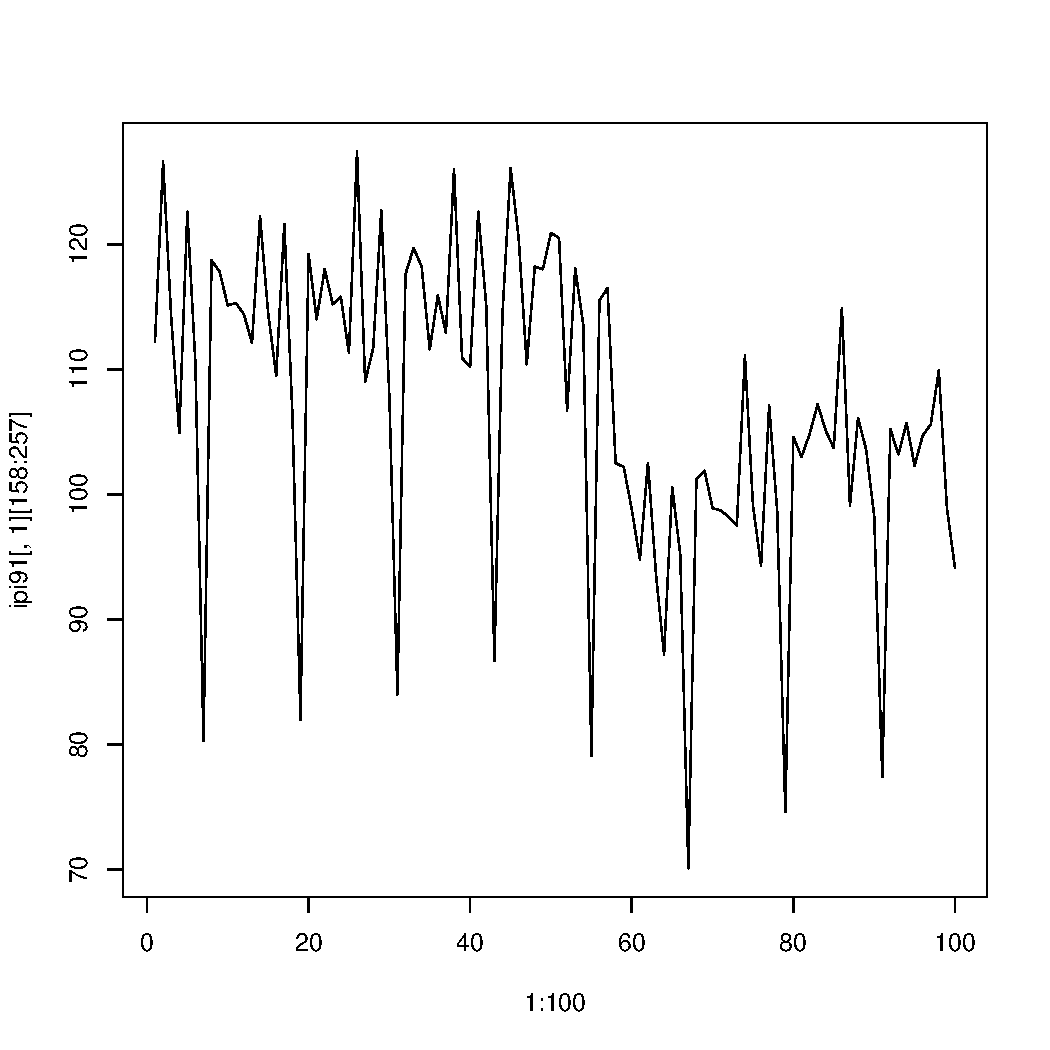
\includegraphics[width=0.5\textwidth]{../imagenes/ipi1original.pdf}}
  \subfloat[Reconstrucción con AR(2)]{
   \label{f:franciaAR}
    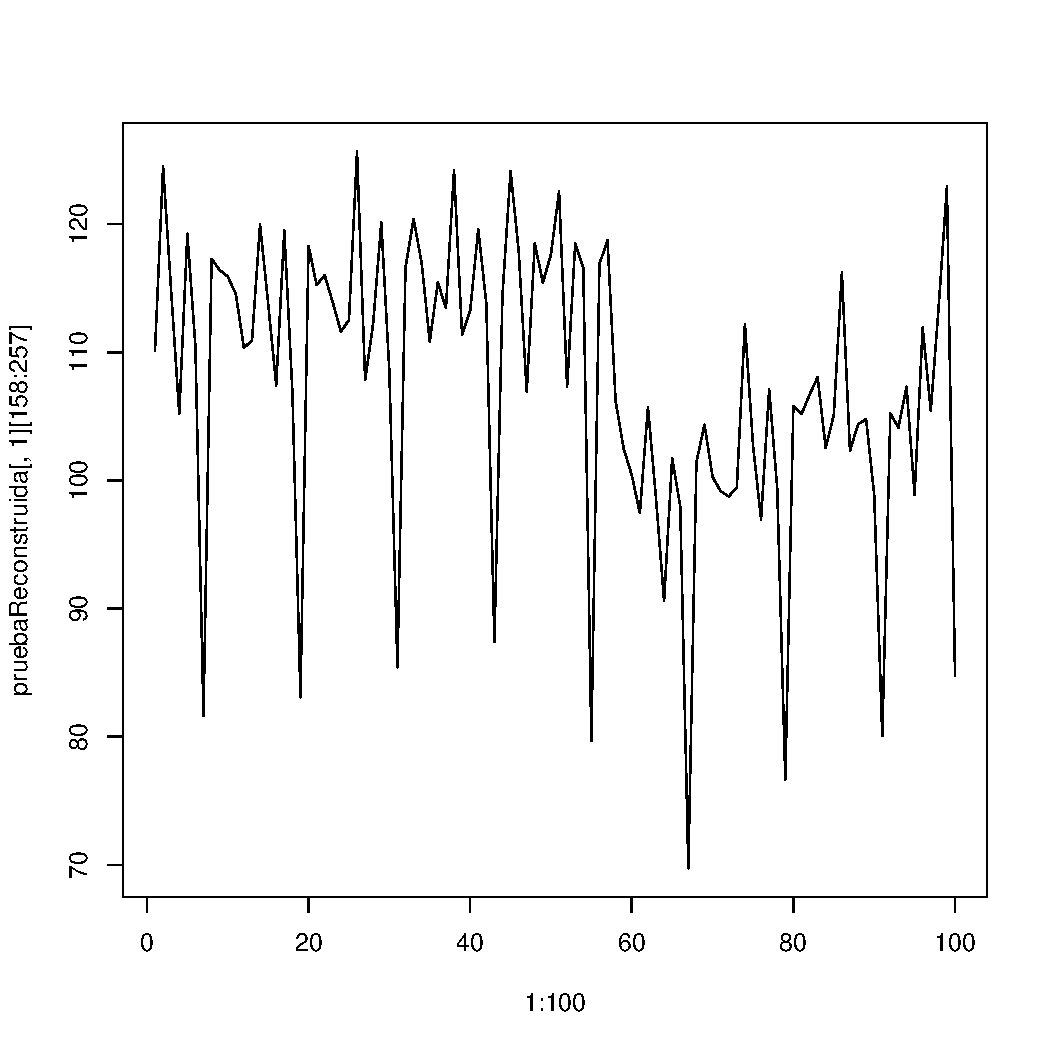
\includegraphics[width=0.5\textwidth]{../imagenes/ipi1ar.pdf}}
    \newline
  \subfloat[Reconstrucción con ARMA(2,2)]{
  \centering
   \label{f:franciaARMA}
    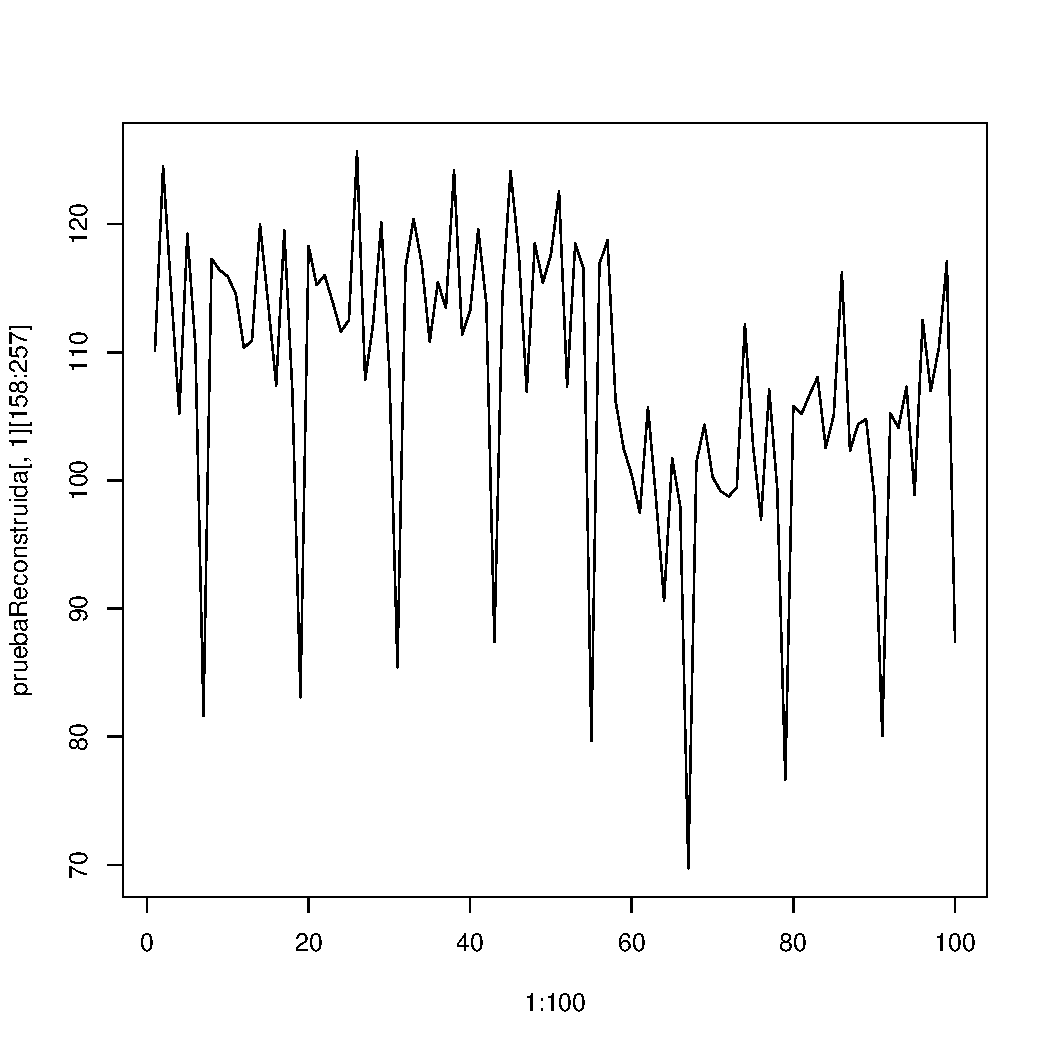
\includegraphics[width=0.5\textwidth]{../imagenes/ipi1arma.pdf}}
 \caption{IPI en Francia}
 \label{f:francia}
\end{figure}

\begin{figure}[]
 \centering
  \subfloat[Serie original]{
   \label{f:alemaniaO}
    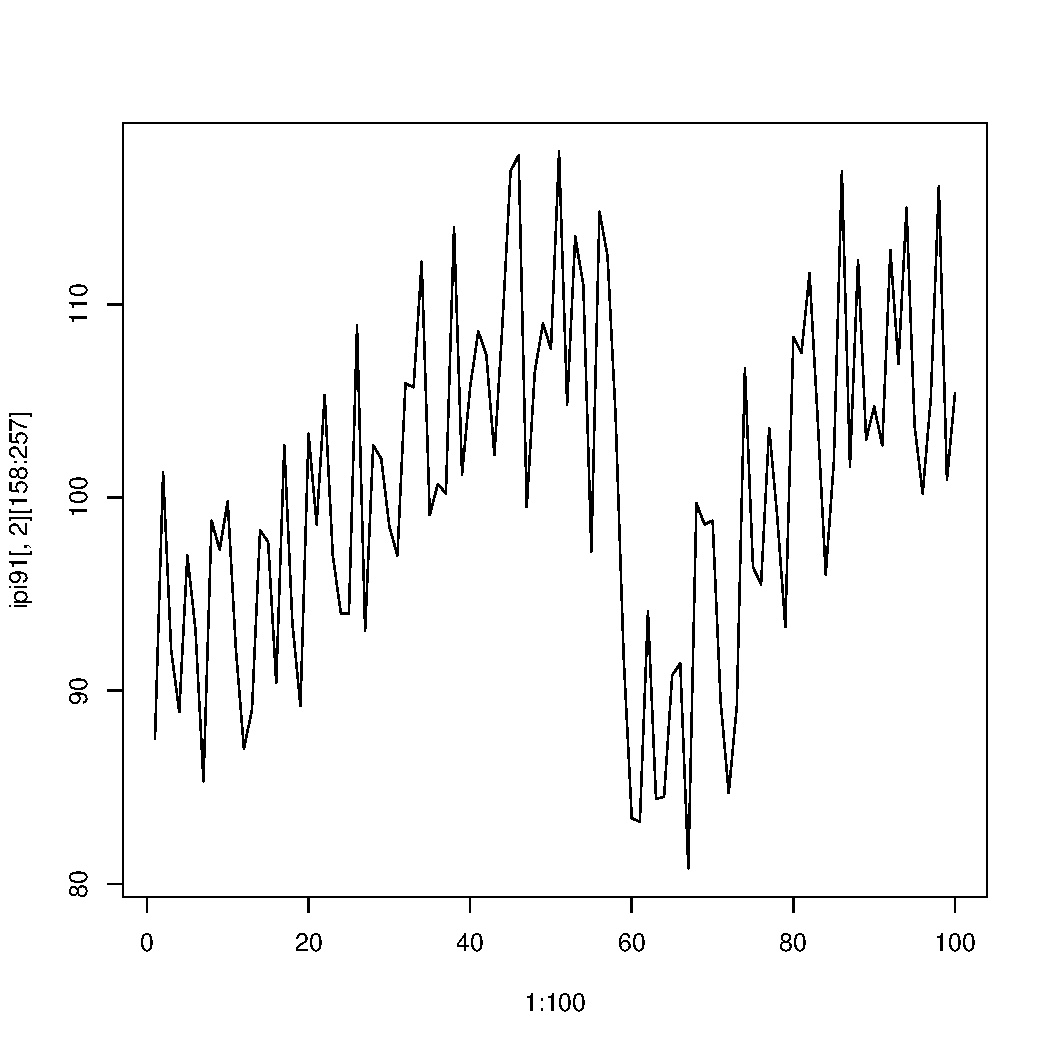
\includegraphics[width=0.5\textwidth]{../imagenes/ipi2original.pdf}}
  \subfloat[Reconstrucción con AR(2)]{
   \label{f:alemaniaAR}
    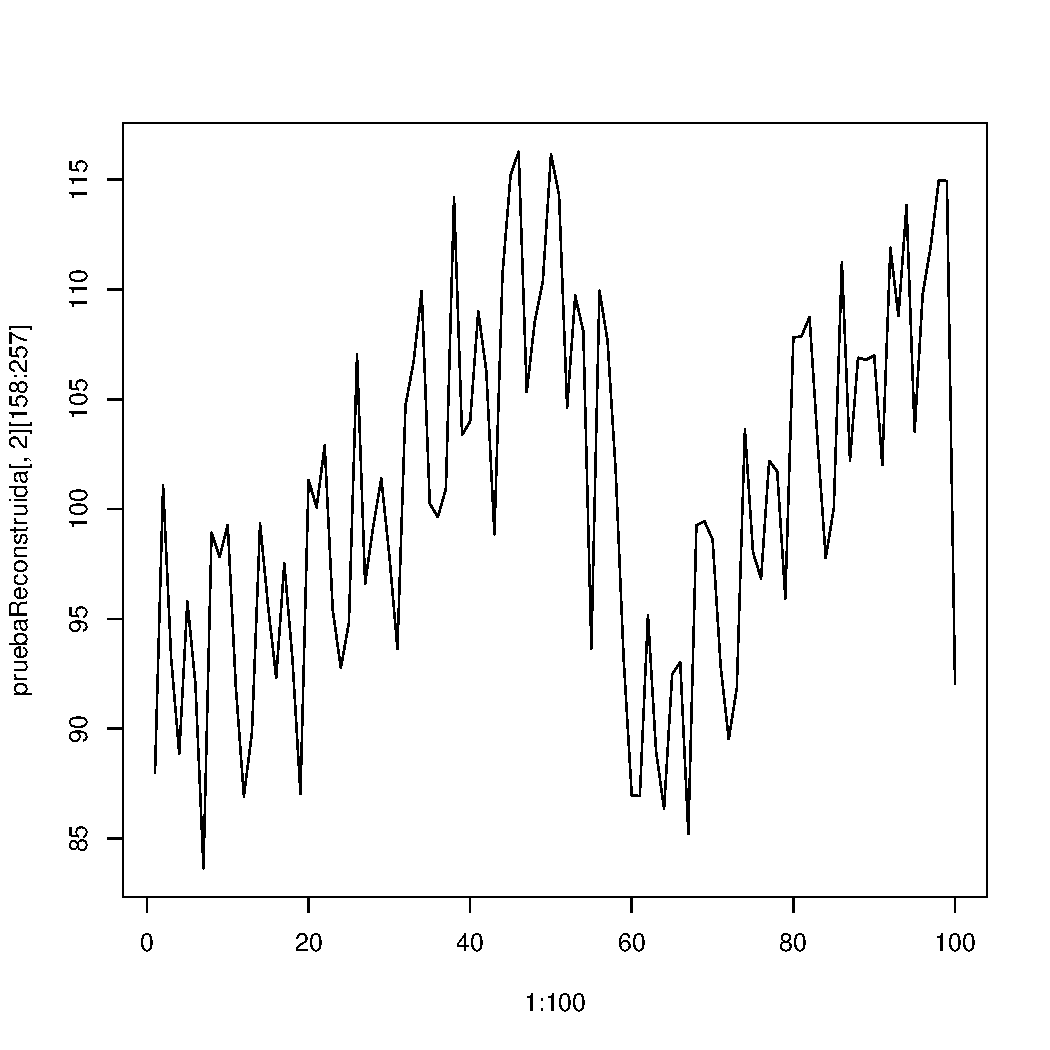
\includegraphics[width=0.5\textwidth]{../imagenes/ipi2ar.pdf}}
    \newline
  \subfloat[Reconstrucción con ARMA(2,2)]{
  \centering
   \label{f:alemaniaARMA}
    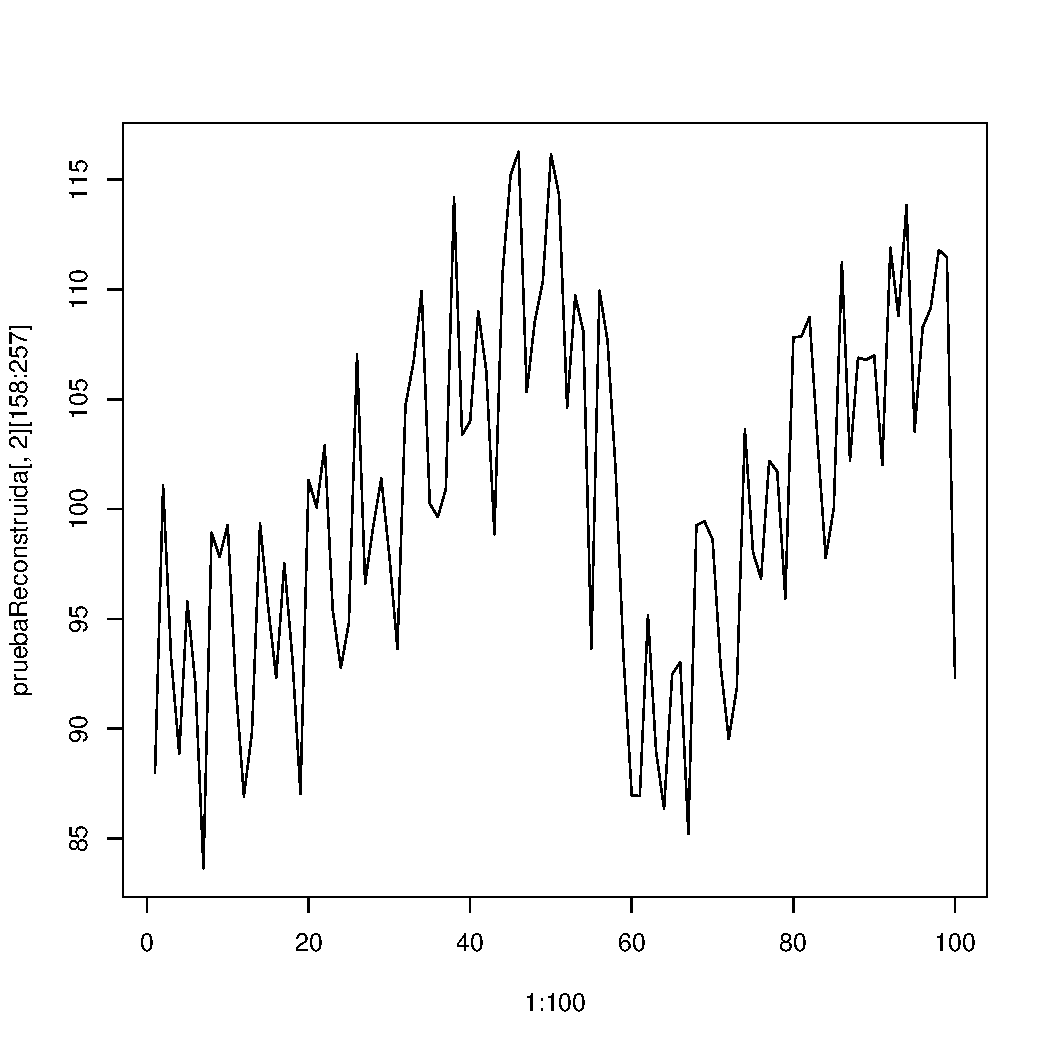
\includegraphics[width=0.5\textwidth]{../imagenes/ipi2arma.pdf}}
 \caption{IPI en Alemania}
 \label{f:alemania}
\end{figure}

\begin{figure}[]
 \centering
  \subfloat[Serie original]{
   \label{f:italiaO}
    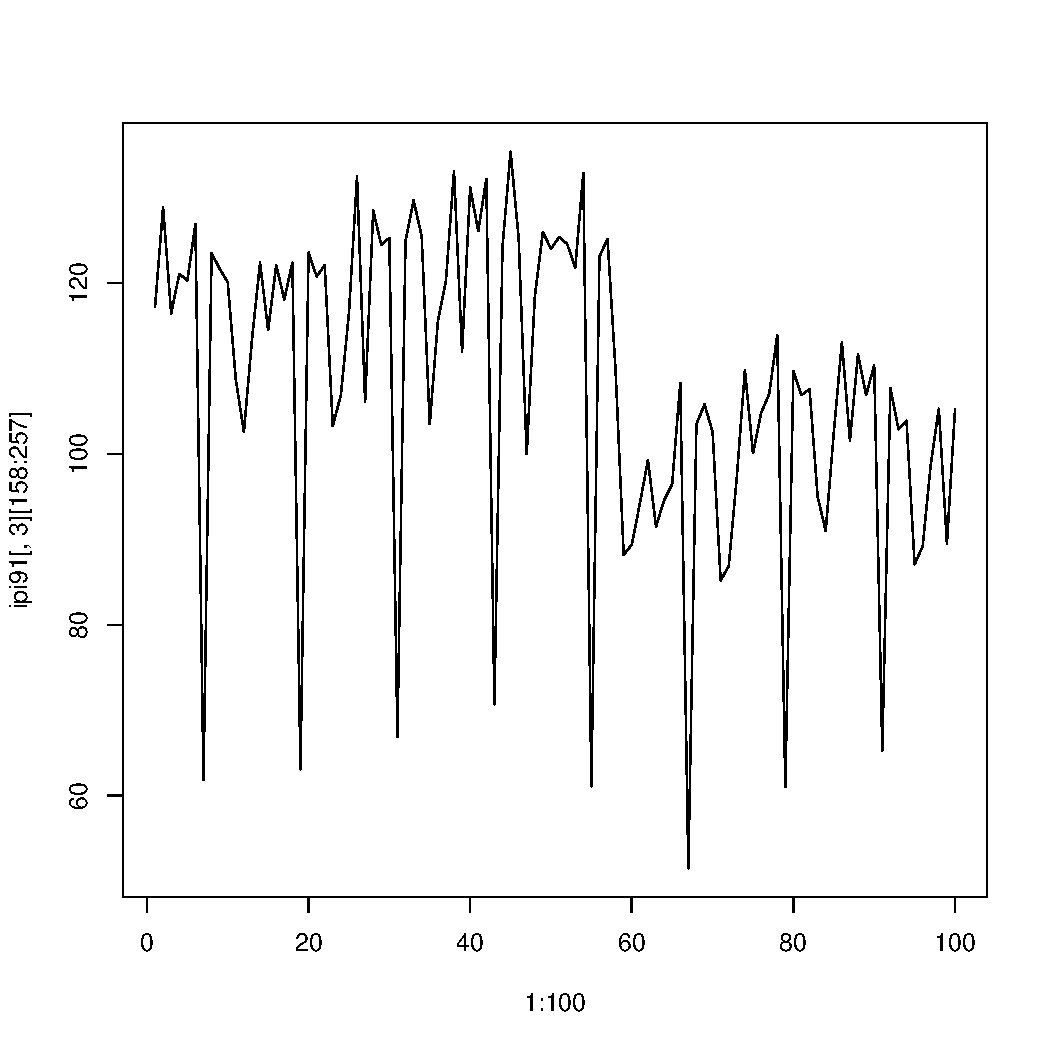
\includegraphics[width=0.5\textwidth]{../imagenes/ipi3original.pdf}}
  \subfloat[Reconstrucción con AR(2)]{
   \label{f:italiaAR}
    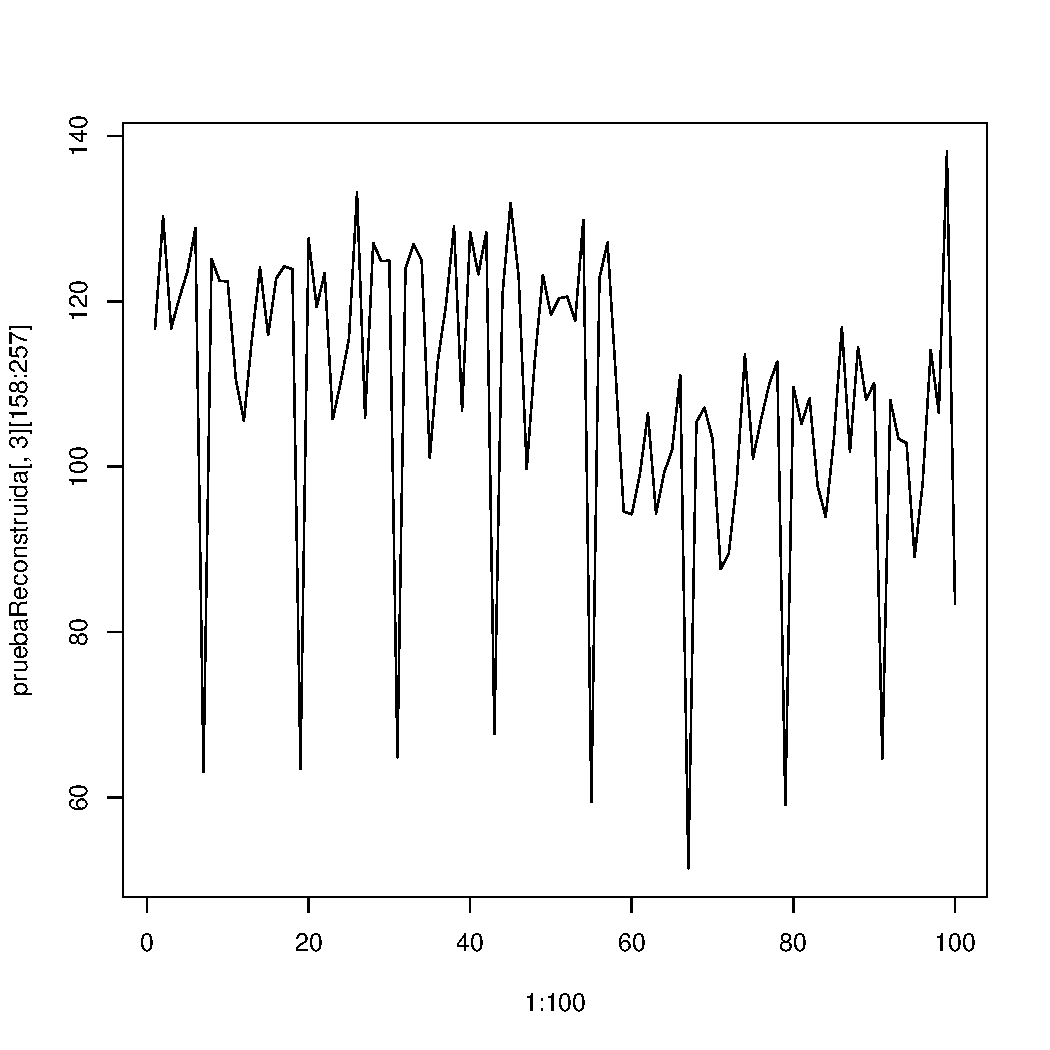
\includegraphics[width=0.5\textwidth]{../imagenes/ipi3ar.pdf}}
    \newline
  \subfloat[Reconstrucción con ARMA(2,2)]{
  \centering
   \label{f:italiaARMA}
    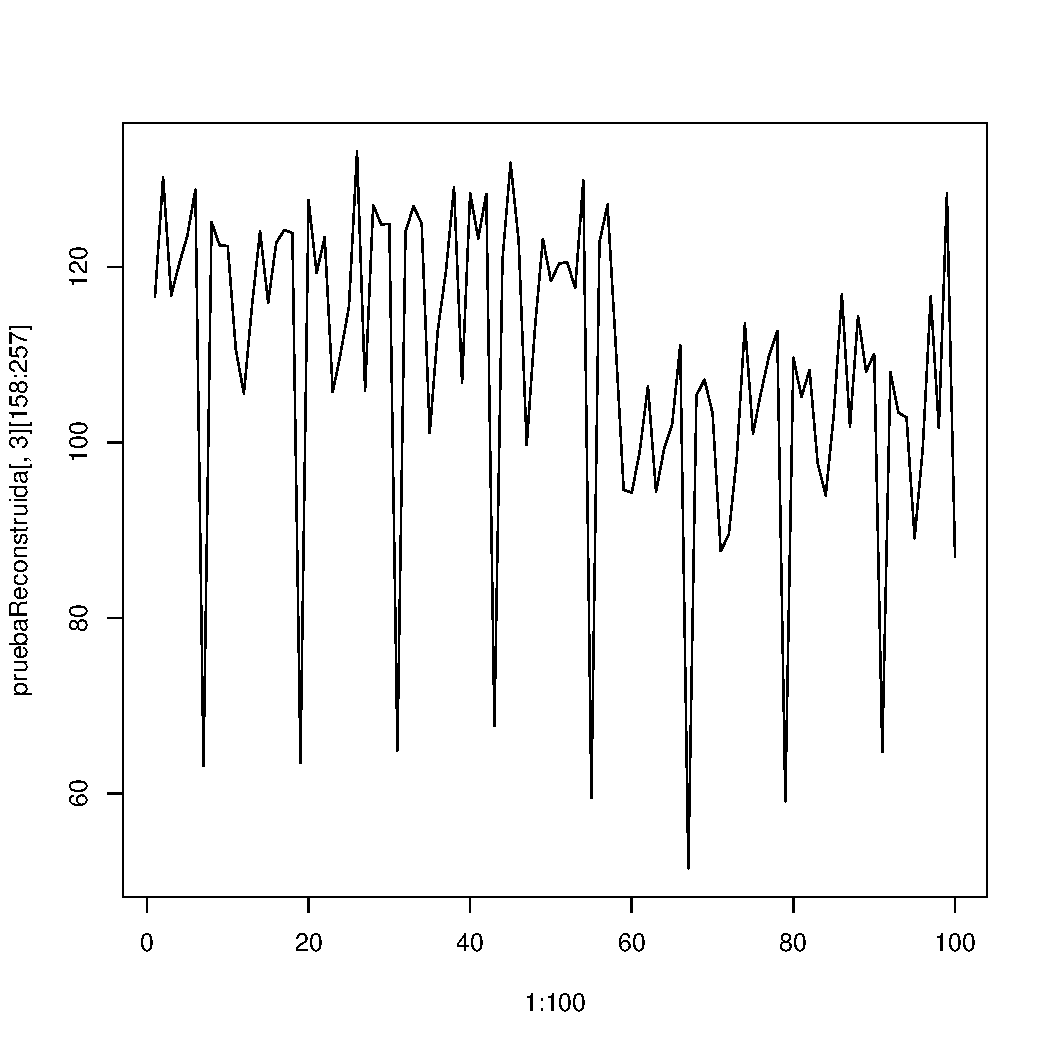
\includegraphics[width=0.5\textwidth]{../imagenes/ipi3arma.pdf}}
 \caption{IPI en Italia}
 \label{f:italia}
\end{figure}

\begin{figure}[]
 \centering
  \subfloat[Serie original]{
   \label{f:ukO}
    \includegraphics[width=0.5\textwidth]{../imagenes/ipi4original.pdf}}
  \subfloat[Reconstrucción con AR(2)]{
   \label{f:ukAR}
    \includegraphics[width=0.5\textwidth]{../imagenes/ipi4ar.pdf}}
    \newline
  \subfloat[Reconstrucción con ARMA(2,2)]{
  \centering
   \label{f:ukARMA}
    \includegraphics[width=0.5\textwidth]{../imagenes/ipi4arma.pdf}}
 \caption{IPI en Reino Unido}
 \label{f:uk}
\end{figure}

En las imágenes apreciamos que el modelo ARMA(2,2) predice la serie un poco mejor que el modelo AR(2). En el caso del modelo AR(2), en la serie del IPI en Francia, se obtiene una diferencia, en valor del absoluto, entre los valores predichos y los originales, de 7.25 en el primer valor predicho, 0.16 en el segundo, 3.85 en el tercero, 24.02 en el cuarto y 9.35 en el quinto. En el caso del modelo ARMA(2,2), estas diferencias son de 7.84, 1.4, 0.44, 18.23 y 6.68. Efectivamente el modelo ARMA(2,2) tiene menos error en esta serie que el modelo AR(2) y vemos que, en general, según vamos aumentando el horizonte de predicción el error va aumentando. Los errores por encima de 10 se consideran altos puesto que los valores de la serie oscilan entre 85 y 115.\\

Para la serie del IPI en Alemania, las diferencias con el modelo AR(2) son de 9.57 en el primer valor predicho, 6.87 en el segundo, 1.12 en el tercero, 14.05 en el cuarto y 13.35 en el quinto. En el caso del modelo ARMA(2,2), las diferencias son de 8.09, 4.05, 4.31, 10.58 y 13.08. En este caso ambos modelos están más igualados pero de nuevo se ve que según se aumenta el horizonte de predicción hay más error.\\

En este caso experimental se han usado modelos sencillos y lineales, pero convendría usar modelos más potentes para obtener unas buenas predicciones de la serie $\mathbf{f}$ y que así los errores en la predicción al volver hacia las series originales se redujeran, siempre teniendo en cuenta que son reconstrucciones utilizando las componentes principales dinámicas, es decir, que se está llevando a cabo una reducción de dimensión con la consiguiente pérdida de información, con lo que siempre va haber un error de base, más allá del que se cometa en la predicción.




%\end{document}
